

\documentclass[10pt,xcolor=dvipsnames]{beamer}\usepackage[]{graphicx}\usepackage[]{color}
%% maxwidth is the original width if it is less than linewidth
%% otherwise use linewidth (to make sure the graphics do not exceed the margin)
\makeatletter
\def\maxwidth{ %
  \ifdim\Gin@nat@width>\linewidth
    \linewidth
  \else
    \Gin@nat@width
  \fi
}
\makeatother

\definecolor{fgcolor}{rgb}{0.345, 0.345, 0.345}
\newcommand{\hlnum}[1]{\textcolor[rgb]{0.686,0.059,0.569}{#1}}%
\newcommand{\hlstr}[1]{\textcolor[rgb]{0.192,0.494,0.8}{#1}}%
\newcommand{\hlcom}[1]{\textcolor[rgb]{0.678,0.584,0.686}{\textit{#1}}}%
\newcommand{\hlopt}[1]{\textcolor[rgb]{0,0,0}{#1}}%
\newcommand{\hlstd}[1]{\textcolor[rgb]{0.345,0.345,0.345}{#1}}%
\newcommand{\hlkwa}[1]{\textcolor[rgb]{0.161,0.373,0.58}{\textbf{#1}}}%
\newcommand{\hlkwb}[1]{\textcolor[rgb]{0.69,0.353,0.396}{#1}}%
\newcommand{\hlkwc}[1]{\textcolor[rgb]{0.333,0.667,0.333}{#1}}%
\newcommand{\hlkwd}[1]{\textcolor[rgb]{0.737,0.353,0.396}{\textbf{#1}}}%
\let\hlipl\hlkwb

\usepackage{framed}
\makeatletter
\newenvironment{kframe}{%
 \def\at@end@of@kframe{}%
 \ifinner\ifhmode%
  \def\at@end@of@kframe{\end{minipage}}%
  \begin{minipage}{\columnwidth}%
 \fi\fi%
 \def\FrameCommand##1{\hskip\@totalleftmargin \hskip-\fboxsep
 \colorbox{shadecolor}{##1}\hskip-\fboxsep
     % There is no \\@totalrightmargin, so:
     \hskip-\linewidth \hskip-\@totalleftmargin \hskip\columnwidth}%
 \MakeFramed {\advance\hsize-\width
   \@totalleftmargin\z@ \linewidth\hsize
   \@setminipage}}%
 {\par\unskip\endMakeFramed%
 \at@end@of@kframe}
\makeatother

\definecolor{shadecolor}{rgb}{.97, .97, .97}
\definecolor{messagecolor}{rgb}{0, 0, 0}
\definecolor{warningcolor}{rgb}{1, 0, 1}
\definecolor{errorcolor}{rgb}{1, 0, 0}
\newenvironment{knitrout}{}{} % an empty environment to be redefined in TeX

\usepackage{alltt}
\setbeamertemplate{navigation symbols}{}



\usepackage{color}
\usepackage{CREAL_slides}
\usepackage[latin1]{inputenc}
\usepackage{calc}
\usepackage[loadonly]{enumitem}
\usepackage{float}
\usepackage[position=top,singlelinecheck=off]{subfig}
\usepackage{amsfonts}
\usepackage{amssymb}
\usepackage{amsmath}
\usepackage{tikz}
\usetikzlibrary{arrows}

\DeclareMathOperator{\argmax}{arg\,max}

\newcommand{\X}{\mathbf{X}}
\newcommand{\ma}[1]{\ensuremath{\mathbf{#1}}}
\newcommand{\y}{\mathbf{y}}
\newcommand{\mba}{\mathbf{a}}


\title[Multivariate methods in health studies]{Integration of muliple tables  \\ \small{in \\ Methods to integrate multiple tables in biomedical studies to detect biomarkers and stratify individuals \\ \medskip
  Instituto de Salud Carlos III. Centro Nacional de Epidemiolog\'ia \\ September, 2017}}
\author[Juan R Gonzalez]{Juan R Gonzalez}
\institute[CREAL]{BRGE - Bioinformatics Research Group in Epidemiology \\
		  Barcelona Institute for Global Health (ISGlobal) \\
		           {\tt e-mail:juanr.gonzalez@isglobal.org} \\
                  \url{http://www.creal.cat/brge} \\
                  and Departament of Mathematics, UAB
                  }

\date{}
\IfFileExists{upquote.sty}{\usepackage{upquote}}{}
\begin{document}




\frame{\titlepage}


\begin{frame}[plain]{Outline}
\tableofcontents
\end{frame}

%%%%%%%%%%%%%%%%%%%%%%%%%%%%%%%%%%%
\section{Introduction}
%%%%%%%%%%%%%%%%%%%%%%%%%%%%%%%%%%%


\begin{frame}[plain]\frametitle{Introduction}

\begin{itemize}
\item Undersanding the genetic basis of \textcolor{OliveGreen}{complex traits} is an open question for may researchers
\pause
\item Recent advances in technology has made this problem even more complex by incorporating other pieces
of information such as neuroimaging, daily measurements of enviromental exposures among others
\pause
\item The main challenge is to analyze the vast amount of data that is being generated, particularly how to integrate information from different tables
\end{itemize}
\end{frame}



\begin{frame}[plain]\frametitle{Introduction}

\begin{figure}
\begin{center}
 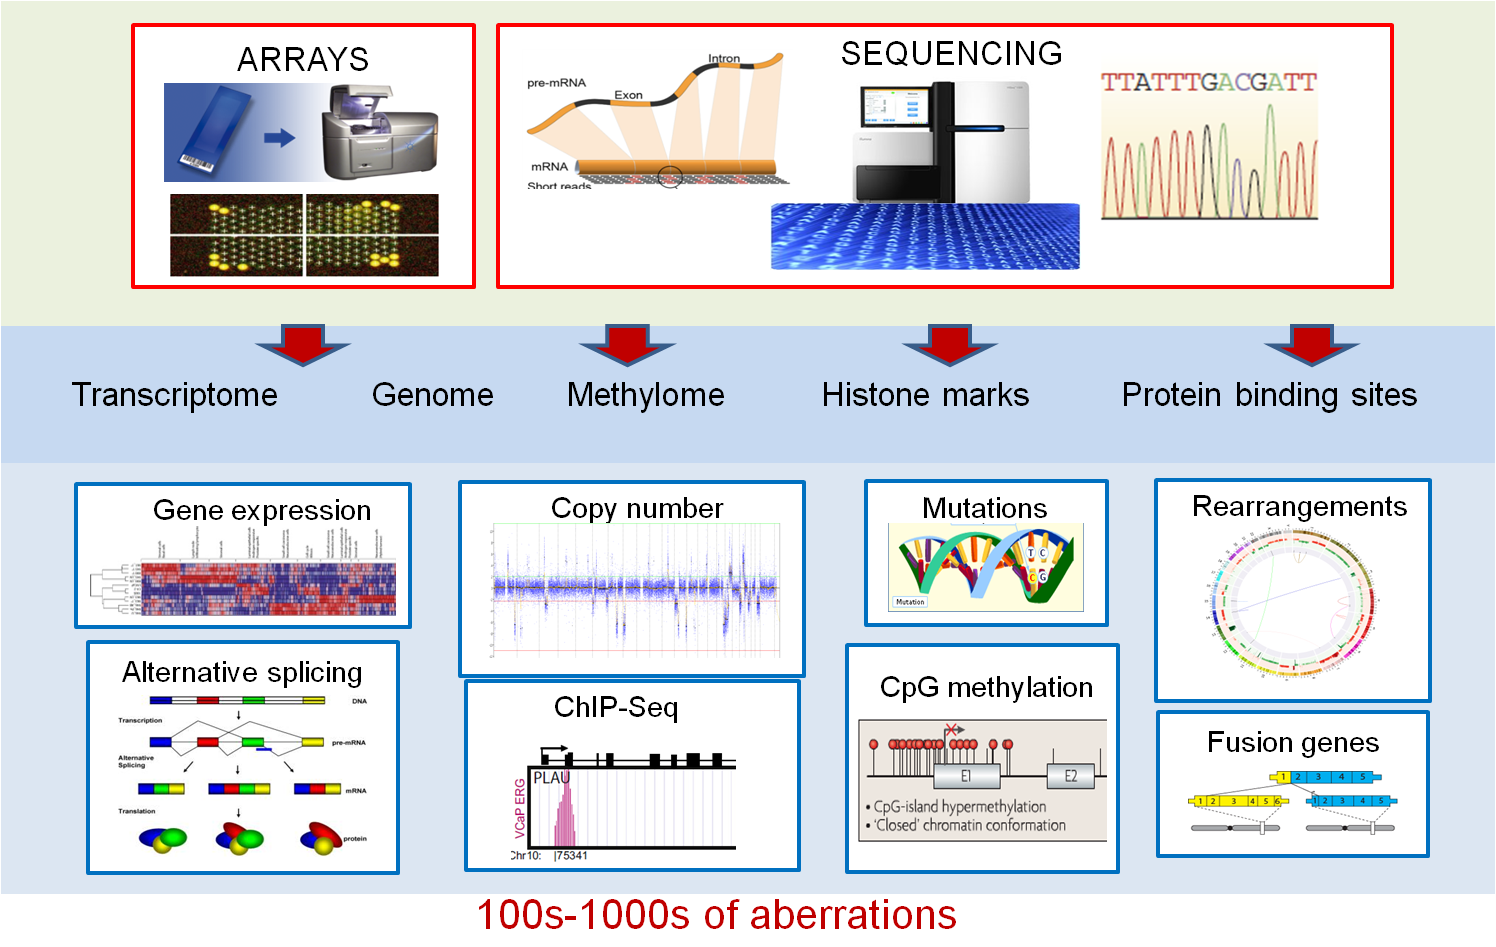
\includegraphics[height=6cm, width=6.5cm]{figures/general_omic_data.png}
\end{center}
\end{figure}

\end{frame}


\begin{frame}[plain]\frametitle{Introduction}

\begin{figure}
\begin{center}
 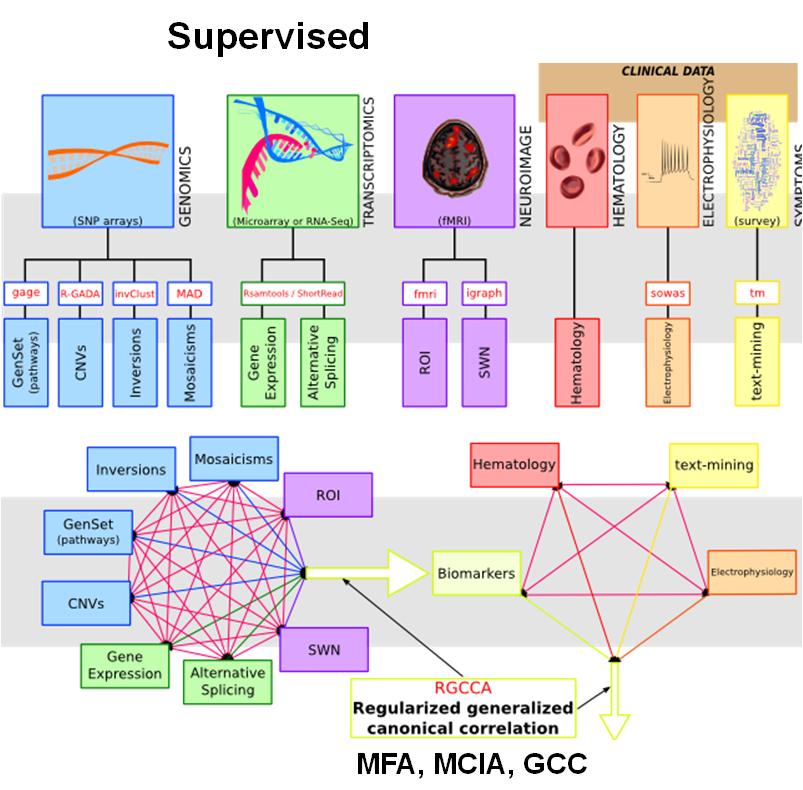
\includegraphics[height=6cm, width=6cm]{figures/supervised_multi_omic.png}
\end{center}
\end{figure}

\end{frame}



\begin{frame}[plain]\frametitle{Introduction}
 \begin{figure}
 \begin{center}
   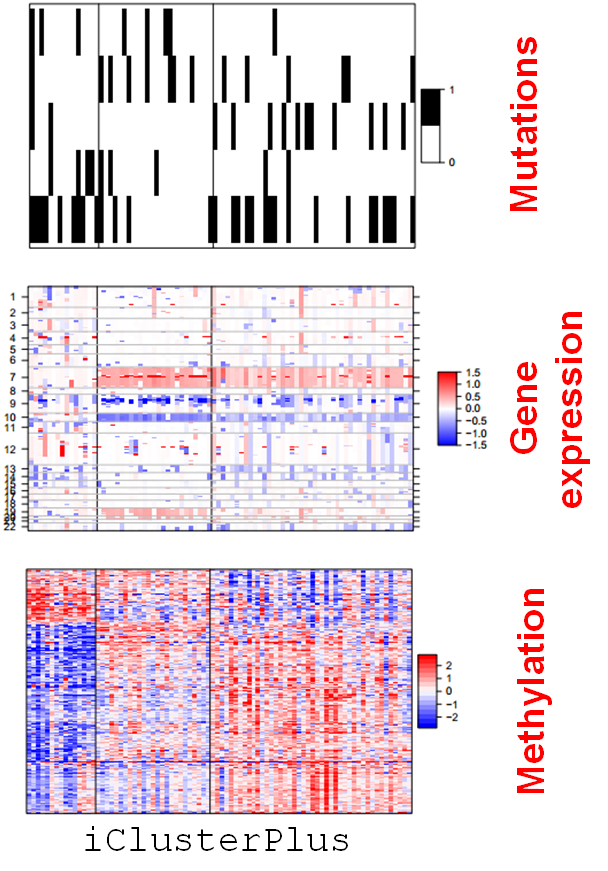
\includegraphics[height=6cm, width=5cm]{figures/non_supervised_multi_omic.png}
  \end{center}
 \end{figure}
\end{frame}



\begin{frame}[plain]\frametitle{Introduction}

\begin{itemize}
\item Data integration (Integrative bioinformatics, integrated
analysis, crossomics, multi-dataset analysis, data fusion, ...) is being crucial in Bioinformatics/Biology/Epidemiology
\item Data integration may refer to different aspects
  \begin{itemize}
   \item Computational combination of data (sets)
   \item Simultaneous analysis of different variables from different tables, different time points, different tissues, ...
   \item Provide biological insights by using information from existing databases (ENCODE, GTEX, KEGG, ...)
  \end{itemize}
\item Here we mean the process by which different types of data are combined as predictor
variables to allow more thorough and comprehensive modelling of complex traits or phenotypes
\end{itemize}
\end{frame}


\begin{frame}[plain]\frametitle{Types of meta-dimensional analyses}

\begin{figure}
\begin{center}
 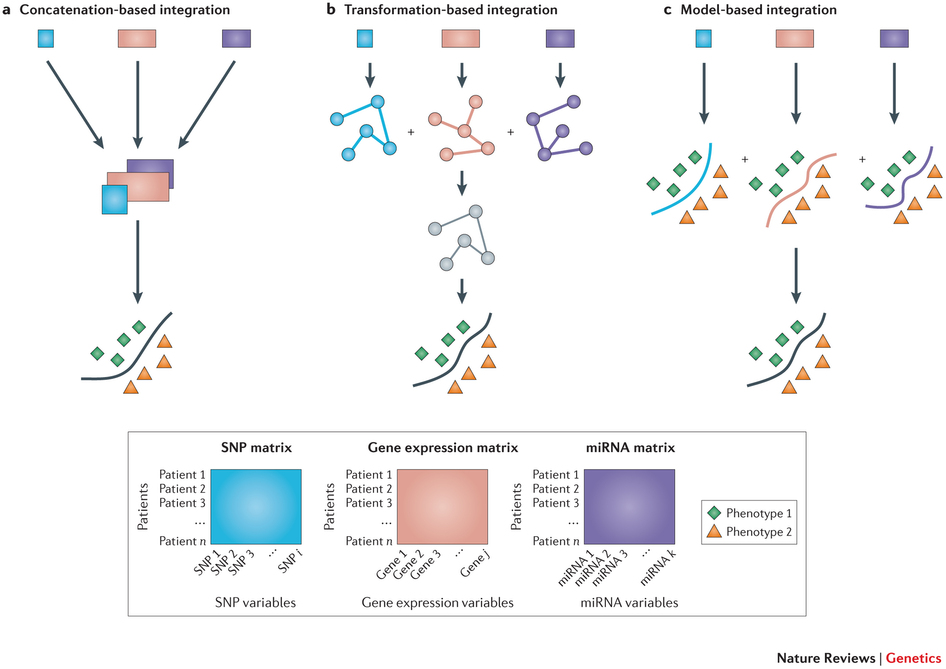
\includegraphics[height=7cm, width=6cm]{figures/meta_dimensional.jpg}
\end{center}
\end{figure}

\end{frame}




\begin{frame}[plain]\frametitle{Mendelian randomization}

\begin{figure}
  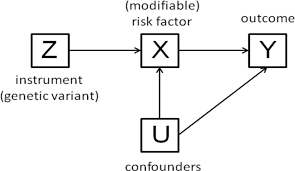
\includegraphics[height=4cm, width=6cm]{figures/mendelian_randomization.png}
\end{figure}

\end{frame}


\begin{frame}[plain]\frametitle{Conditional Tests}

\begin{figure}
  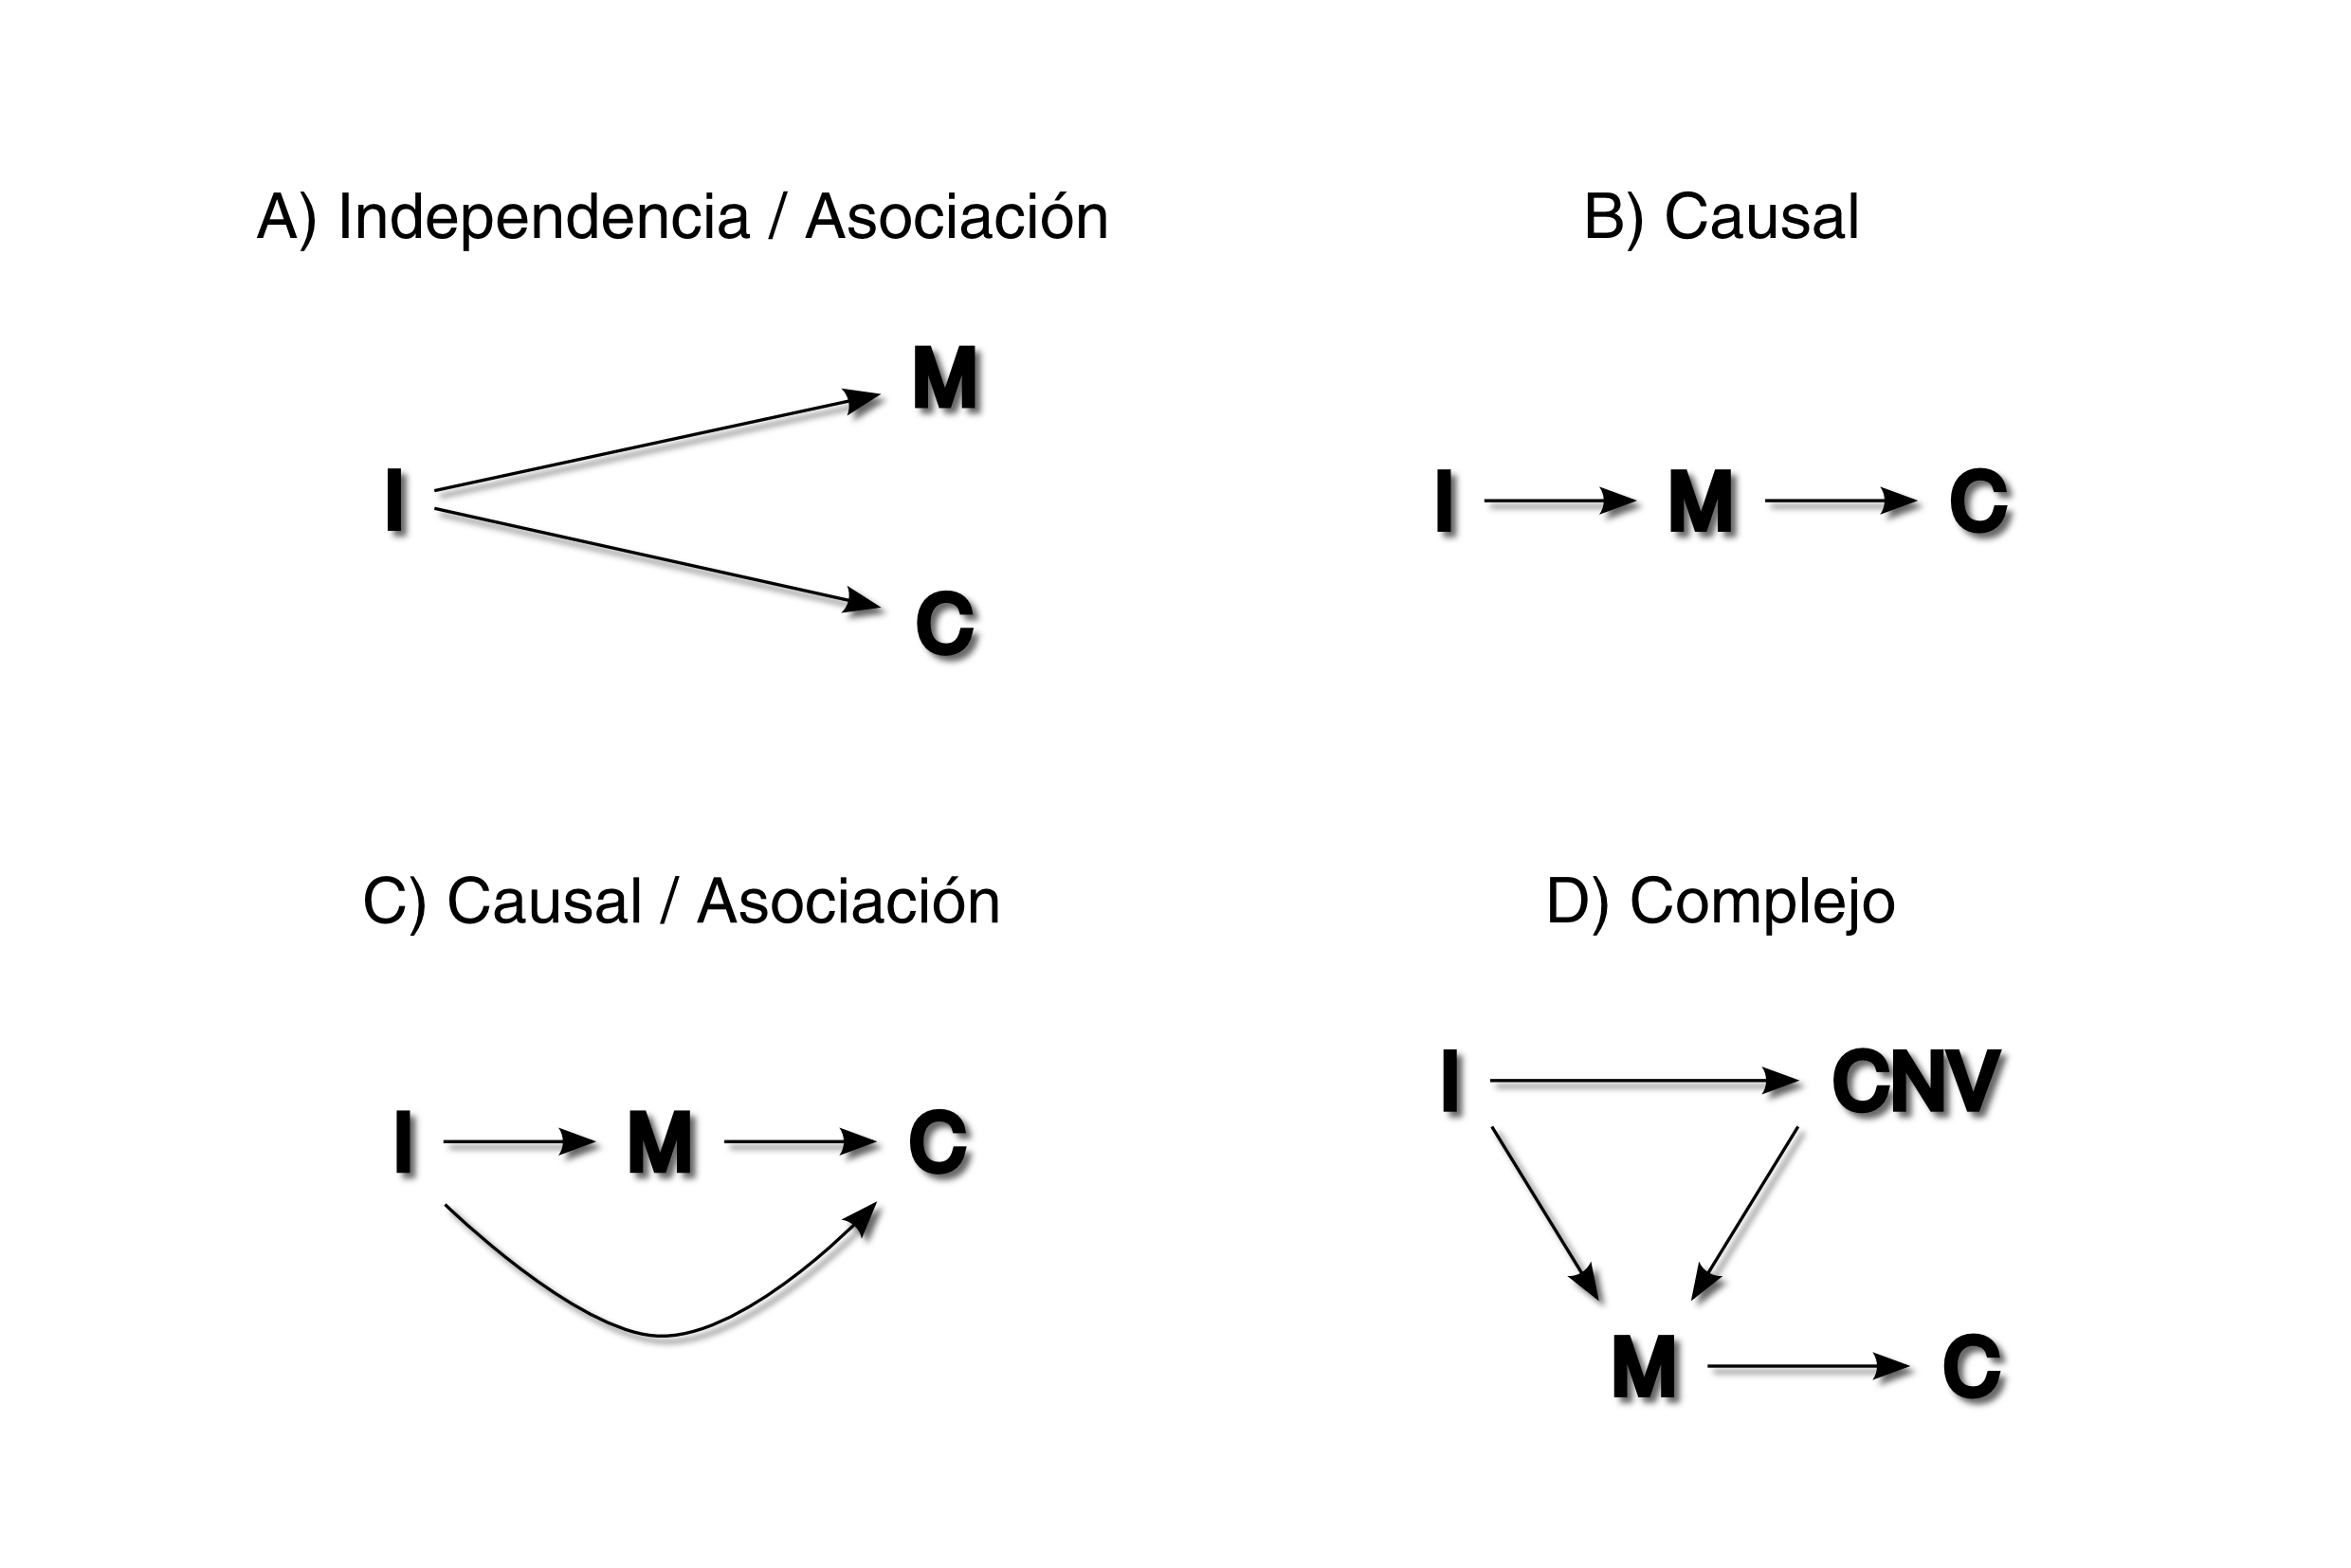
\includegraphics[height=5cm, width=7cm]{figures/CIT.png}
\end{figure}

\end{frame}


%%%%%%%%%%%%%%%%%%%%%%%%%%%%%%%%%%%
\section{Integrating two or more omic datasets}
%%%%%%%%%%%%%%%%%%%%%%%%%%%%%%%%%%%



\begin{frame}[plain]\frametitle{Multiple dataset: dimensionality reduction}

\begin{figure}
\begin{center}
 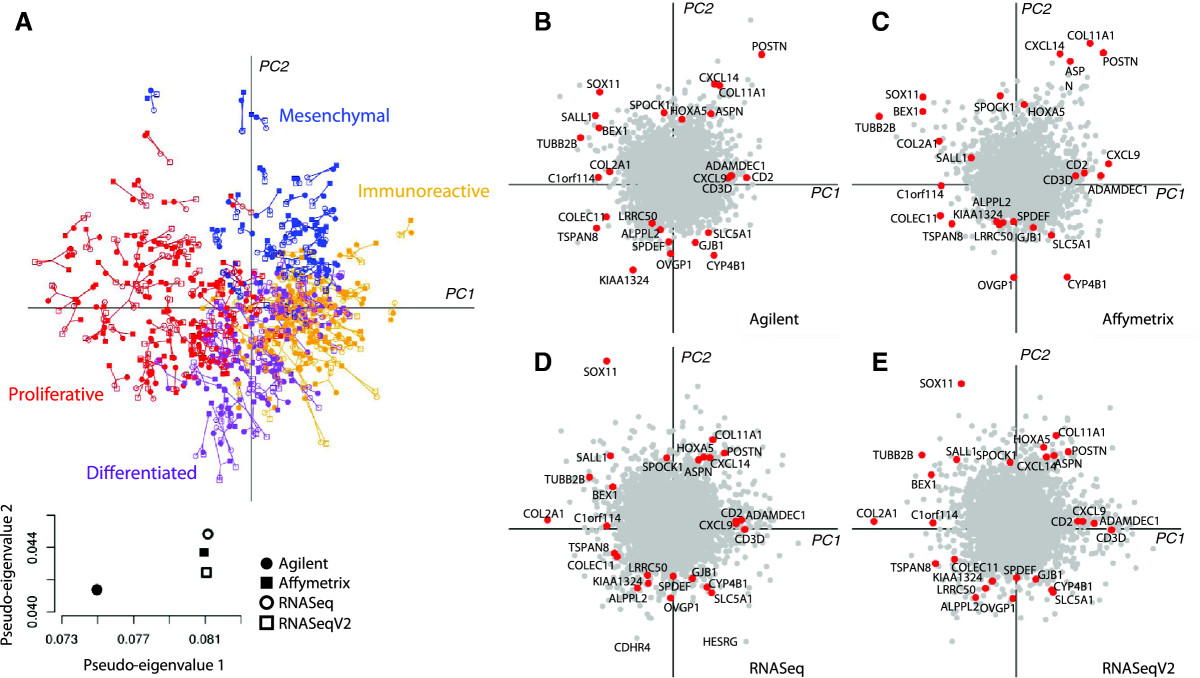
\includegraphics[height=5.5cm, width=6cm]{figures/multi_example.jpg}
\end{center}
\end{figure}

\end{frame}


\begin{frame}[plain]\frametitle{Integrating two or more datasets}

\begin{itemize}
\item There are methods based on dimension reduction techniques: generalized SVD, Co-Inertia Analysis (CIA), sparse or penalized extensions of Partial Least Squares (PLS),
Canonical Correlation (CCA), Multiple Factor Analysis (MFA), Generalized Canonical Correlation (GCA)
\pause
\item There are methods that are based on path modelling: structural equation models (SEM)
\pause
\item Reguralized Generalized Canonical Correlation (RGCA) provides a unified framework for different approaches (Tenenhaus, M. and Tenenhaus, A. Psychometrika, 2011, 76(2):257-284). Other methods are special cases of RGCA.
\pause
\item RGCA integrates a feature selection method, named sparse GCCA (SGCCA) (Tenenhaus, A et al. Biostatistics, 2014, 15(3):569-83).
\end{itemize}

\end{frame}




\begin{frame}[plain]\frametitle{Integrating two or more datasets}

\begin{itemize}
\item Canonical Correlation can be seen as an extension of PCA for more than two tables $X$ and $Y$
\item The two datasets can be decomposed as:
$$ f =Xp $$ $$ g =Yq $$
where $p$ and $q$ are the loading vectors
\item CCA searches for association or correlations among $X$ and $Y$ by
$$ \argmax_{p^i q^i} \text{cor}(Xp^i Yq^i)$$
for the $i$-th component
\item $Xp^i$ and $Yq^i$ are known as canonical variates and their correlations are the canonical correlations.
\end{itemize}

\end{frame}


\begin{frame}[plain]{Integrating two or more datasets}

\begin{itemize}
\item ($p >> n$) is an issue. Additionally, there is often presence of multicollinearity within both sets of variables that requires a reguralization step.
\item This may accomplished by addign a ridge penalty, that is, adding a multiple of the identity matrix to the correlation/covariance matrix.
$$ \argmax_{p^i q^i} \text{cor}(Xp^i Yq^i) + \lambda \text{I}$$

\item A sparse solution (filtering the number of variables) is the solution: pCCA, sCCA, CCA-l1, CCA-EN, CCA-group sparse have been used to integrate two omic data.
\end{itemize}
\end{frame}



\begin{frame}[plain]\frametitle{Integrating two or more datasets}

\begin{figure}
\begin{center}
 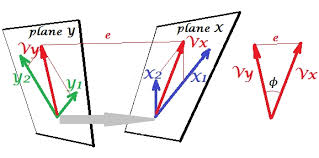
\includegraphics[height=3.5cm, width=6cm]{figures/canonical_correlation.jpg}
\end{center}
\end{figure}

$V_y$ and $V_x$ are selected to maximize:

\begin{itemize}
 \item Correlation (CCA)
 \item Squared Covariance (CIA)
       $$ \argmax_{p^i q^i} \text{cov}^2(Xp^i Yq^i)$$
\end{itemize}

\end{frame}

\begin{frame}[plain]\frametitle{Canonical Correlation}

\begin{itemize}
\item CCA has been used in omic data
\item The main limitation is that the number of features generally greatly exceeds the number of observations
\item Consequence 1: parameter estimation cannot be applied using standard methods
\item  Consequence 2: Most of markers are having no effect in the canonical axes (e.g. almost all components in a and b are 0)
\item Penalized (sparse) CCA has been proposed
\item Main advantages: More than two tables, easy interpretation (do not need computing p-values nor correcting for multiple comparisons)
\end{itemize}

\end{frame}



\begin{frame}[plain]\frametitle{Sparse canonical correlation}

\begin{figure}
\begin{center}
 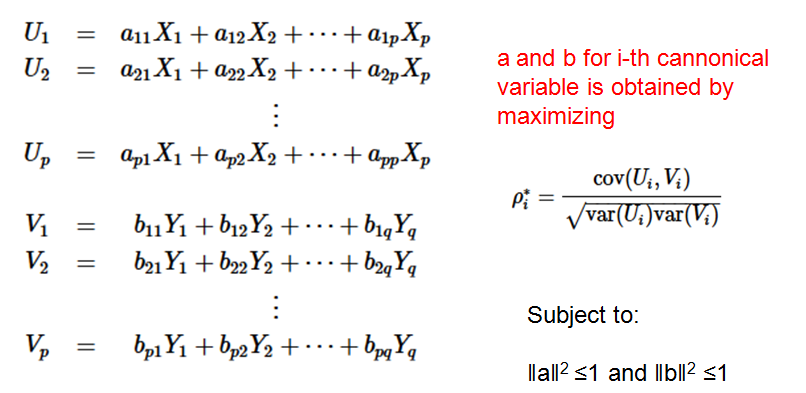
\includegraphics[height=5cm, width=8cm]{figures/mCCA.png}
\end{center}
\end{figure}

\end{frame}

\begin{frame}[plain]{Co-Inertia}

\begin{itemize}

  \item CIA does not requires an inversion step of the covariance matrix; thus, regularization or penalization implementation is not required
  \item CIA can deal with disperse variables
  \item CIA does consider quantitative or qualitative variables
  \item Can weight cases
  \item The method provides the RV coefficient. This is a measure of global similarity between the datasets, and is a number between 0 and 1. The closer it is to 1 the greater the global similarity between the two datasets.
 \end{itemize}

\end{frame}



\begin{frame}[fragile, plain]{Data analysis illustration}

\begin{itemize}
  \item Data from the Cancer Genome Atlas (TCGA) will be analyzed.
  \item A subset of the TCGA breast cancer study from Nature 2012 publication have been selected.
  \item Data {\tt https://tcga-data.nci.nih.gov/docs/publications/brca\_2012/}.
  \item Available data are: miRNA, miRNAprecursor, RNAseq, Methylation, proteins from a RPPA array, and  GISTIC SNP calls (CNA and LOH). Clinical data are also available.
  \item We are interested in comparing women with ER+ vs ER-.
 \end{itemize}
\begin{knitrout}\footnotesize
\definecolor{shadecolor}{rgb}{0.969, 0.969, 0.969}\color{fgcolor}\begin{kframe}
\begin{alltt}
\hlkwd{load}\hlstd{(}\hlstr{"data/breast_TCGA.RData"}\hlstd{)}
\hlstd{group} \hlkwb{<-} \hlkwd{droplevels}\hlstd{(breast_multi}\hlopt{$}\hlstd{clin}\hlopt{$}\hlstd{ER.Status)}
\end{alltt}
\end{kframe}
\end{knitrout}
\end{frame}



\begin{frame}[fragile, plain]\frametitle{Canonical Correlation: gene expression and proteins}

\begin{knitrout}\footnotesize
\definecolor{shadecolor}{rgb}{0.969, 0.969, 0.969}\color{fgcolor}\begin{kframe}
\begin{alltt}
\hlkwd{require}\hlstd{(CCA)}
\hlstd{df1} \hlkwb{<-} \hlkwd{t}\hlstd{(breast_multi}\hlopt{$}\hlstd{RNAseq)[,}\hlnum{1}\hlopt{:}\hlnum{1000}\hlstd{]}
\hlstd{df2} \hlkwb{<-} \hlkwd{t}\hlstd{(breast_multi}\hlopt{$}\hlstd{RPPA)}
\end{alltt}
\end{kframe}
\end{knitrout}

\begin{knitrout}\footnotesize
\definecolor{shadecolor}{rgb}{0.969, 0.969, 0.969}\color{fgcolor}\begin{kframe}
\begin{alltt}
\hlstd{resCC} \hlkwb{<-} \hlkwd{cc}\hlstd{(df1, df2)}
\end{alltt}
\end{kframe}
\end{knitrout}


\begin{verbatim}
Error en chol.default(Bmat) :
  la submatriz de orden 81 no es definida positiva
\end{verbatim}

\begin{knitrout}\footnotesize
\definecolor{shadecolor}{rgb}{0.969, 0.969, 0.969}\color{fgcolor}\begin{kframe}
\begin{alltt}
\hlstd{resRCC} \hlkwb{<-} \hlkwd{rcc}\hlstd{(df1, df2,} \hlnum{0.2}\hlstd{,} \hlnum{0.1}\hlstd{)}
\end{alltt}
\end{kframe}
\end{knitrout}

\begin{knitrout}\footnotesize
\definecolor{shadecolor}{rgb}{0.969, 0.969, 0.969}\color{fgcolor}\begin{kframe}
\begin{alltt}
\hlstd{regul} \hlkwb{<-} \hlkwd{estim.regul}\hlstd{(df1, df2)}
\hlstd{resRCC2} \hlkwb{<-} \hlkwd{rcc}\hlstd{(df1, df2, regul}\hlopt{$}\hlstd{lambda1, regul}\hlopt{$}\hlstd{lambda2)}
\end{alltt}
\end{kframe}
\end{knitrout}

\begin{knitrout}\footnotesize
\definecolor{shadecolor}{rgb}{0.969, 0.969, 0.969}\color{fgcolor}\begin{kframe}
\begin{alltt}
\hlkwd{plt.cc}\hlstd{(resRCC)}
\end{alltt}
\end{kframe}
\end{knitrout}

\end{frame}


\begin{frame}[fragile, plain]\frametitle{Canonical Correlation: gene expression and proteins}

\begin{knitrout}\footnotesize
\definecolor{shadecolor}{rgb}{0.969, 0.969, 0.969}\color{fgcolor}

{\centering 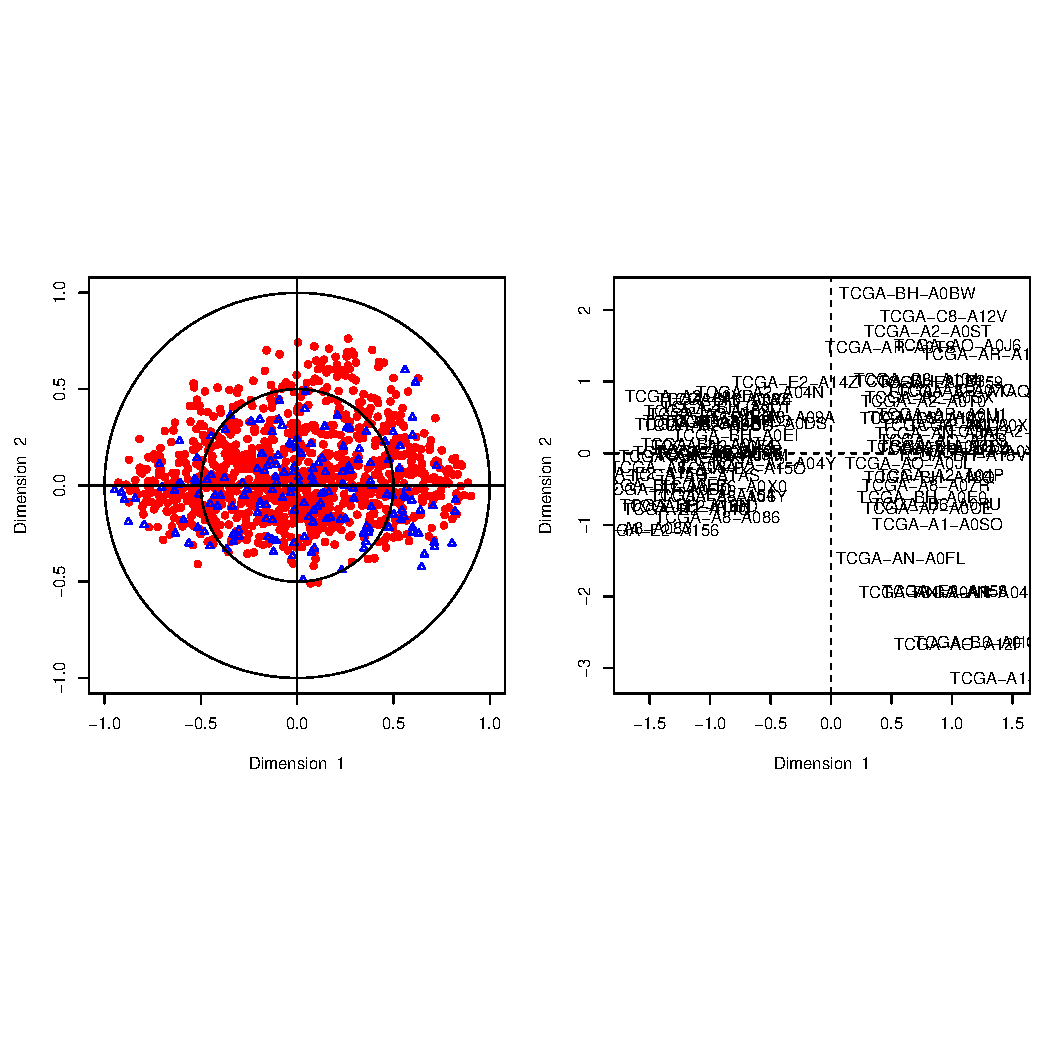
\includegraphics[width=2in]{figure/plot_rcc_out-1} 

}



\end{knitrout}

\end{frame}




\begin{frame}[fragile, plain]\frametitle{Canonical Correlation: gene expression and proteins}


\begin{knitrout}\footnotesize
\definecolor{shadecolor}{rgb}{0.969, 0.969, 0.969}\color{fgcolor}\begin{kframe}
\begin{alltt}
\hlkwd{require}\hlstd{(PMA)}
\hlstd{ddlist} \hlkwb{<-} \hlkwd{list}\hlstd{(df1, df2)}
\hlstd{perm.out} \hlkwb{<-} \hlkwd{MultiCCA.permute}\hlstd{(ddlist,}
                             \hlkwc{type}\hlstd{=}\hlkwd{c}\hlstd{(}\hlstr{"standard"}\hlstd{,} \hlstr{"standard"}\hlstd{),}
                             \hlkwc{trace}\hlstd{=}\hlnum{FALSE}\hlstd{)}
\end{alltt}
\end{kframe}
\begin{kframe}\begin{alltt}
\hlstd{resMultiCCA} \hlkwb{<-} \hlkwd{MultiCCA}\hlstd{(ddlist,}
                        \hlkwc{penalty}\hlstd{=perm.out}\hlopt{$}\hlstd{bestpenalties,}
                        \hlkwc{ws}\hlstd{=perm.out}\hlopt{$}\hlstd{ws.init,}
                        \hlkwc{type}\hlstd{=}\hlkwd{c}\hlstd{(}\hlstr{"standard"}\hlstd{,} \hlstr{"standard"}\hlstd{),}
                        \hlkwc{ncomponents}\hlstd{=}\hlnum{1}\hlstd{,} \hlkwc{trace}\hlstd{=}\hlnum{FALSE}\hlstd{,} \hlkwc{standardize}\hlstd{=}\hlnum{TRUE}\hlstd{)}
\end{alltt}
\end{kframe}
\end{knitrout}

NOTE: setting {\tt type} equal to "ordered" allows to consider that features are correlated (e.g. genomic regions)
\end{frame}


\begin{frame}[fragile, plain]\frametitle{Canonical Correlation: gene expression and proteins}

\begin{knitrout}\scriptsize
\definecolor{shadecolor}{rgb}{0.969, 0.969, 0.969}\color{fgcolor}\begin{kframe}
\begin{alltt}
\hlkwd{rownames}\hlstd{(resMultiCCA}\hlopt{$}\hlstd{ws[[}\hlnum{1}\hlstd{]])} \hlkwb{<-} \hlkwd{colnames}\hlstd{(df1)}
\hlkwd{rownames}\hlstd{(resMultiCCA}\hlopt{$}\hlstd{ws[[}\hlnum{2}\hlstd{]])} \hlkwb{<-} \hlkwd{colnames}\hlstd{(df2)}
\hlkwd{head}\hlstd{(resMultiCCA}\hlopt{$}\hlstd{ws[[}\hlnum{1}\hlstd{]])}
\end{alltt}
\begin{verbatim}
##                  [,1]
## CREB3L1   0.030502191
## PNMA1     0.035339312
## MMP2      0.000000000
## C10orf90 -0.009616231
## GPR98     0.049652420
## APBB2     0.084521773
\end{verbatim}
\begin{alltt}
\hlkwd{head}\hlstd{(resMultiCCA}\hlopt{$}\hlstd{ws[[}\hlnum{2}\hlstd{]])}
\end{alltt}
\begin{verbatim}
##                    [,1]
## c.Myc       -0.03022533
## HER3         0.00000000
## XBP1         0.00000000
## Fibronectin  0.00000000
## PAI.1        0.00000000
## p21          0.00000000
\end{verbatim}
\end{kframe}
\end{knitrout}

NOTE: we are interested in selecting those features having a coefficient (\texttt{ws}) different from 0.

\end{frame}





\begin{frame}[fragile, plain]\frametitle{Co-inertia: gene expression and proteins}

Let us load required packages (coinertia and multiple coinertia)
\begin{knitrout}\footnotesize
\definecolor{shadecolor}{rgb}{0.969, 0.969, 0.969}\color{fgcolor}\begin{kframe}
\begin{alltt}
\hlkwd{library}\hlstd{(made4)}
\hlkwd{library}\hlstd{(omicade4)}
\end{alltt}
\end{kframe}
\end{knitrout}

\begin{knitrout}\footnotesize
\definecolor{shadecolor}{rgb}{0.969, 0.969, 0.969}\color{fgcolor}\begin{kframe}
\begin{alltt}
\hlstd{resCIA} \hlkwb{<-} \hlkwd{cia}\hlstd{(breast_multi}\hlopt{$}\hlstd{RNAseq, breast_multi}\hlopt{$}\hlstd{RPPA)}
\end{alltt}
\end{kframe}
\end{knitrout}

\begin{knitrout}\footnotesize
\definecolor{shadecolor}{rgb}{0.969, 0.969, 0.969}\color{fgcolor}\begin{kframe}
\begin{alltt}
\hlkwd{plot}\hlstd{(resCIA,} \hlkwc{classvec}\hlstd{=group,} \hlkwc{nlab}\hlstd{=}\hlnum{3}\hlstd{,} \hlkwc{clab}\hlstd{=}\hlnum{0}\hlstd{,} \hlkwc{cpoint}\hlstd{=}\hlnum{3} \hlstd{)}
\end{alltt}
\end{kframe}
\end{knitrout}

\end{frame}



\begin{frame}[fragile, plain]\frametitle{Co-inertia: gene expression and proteins}

\begin{figure}
\begin{center}
 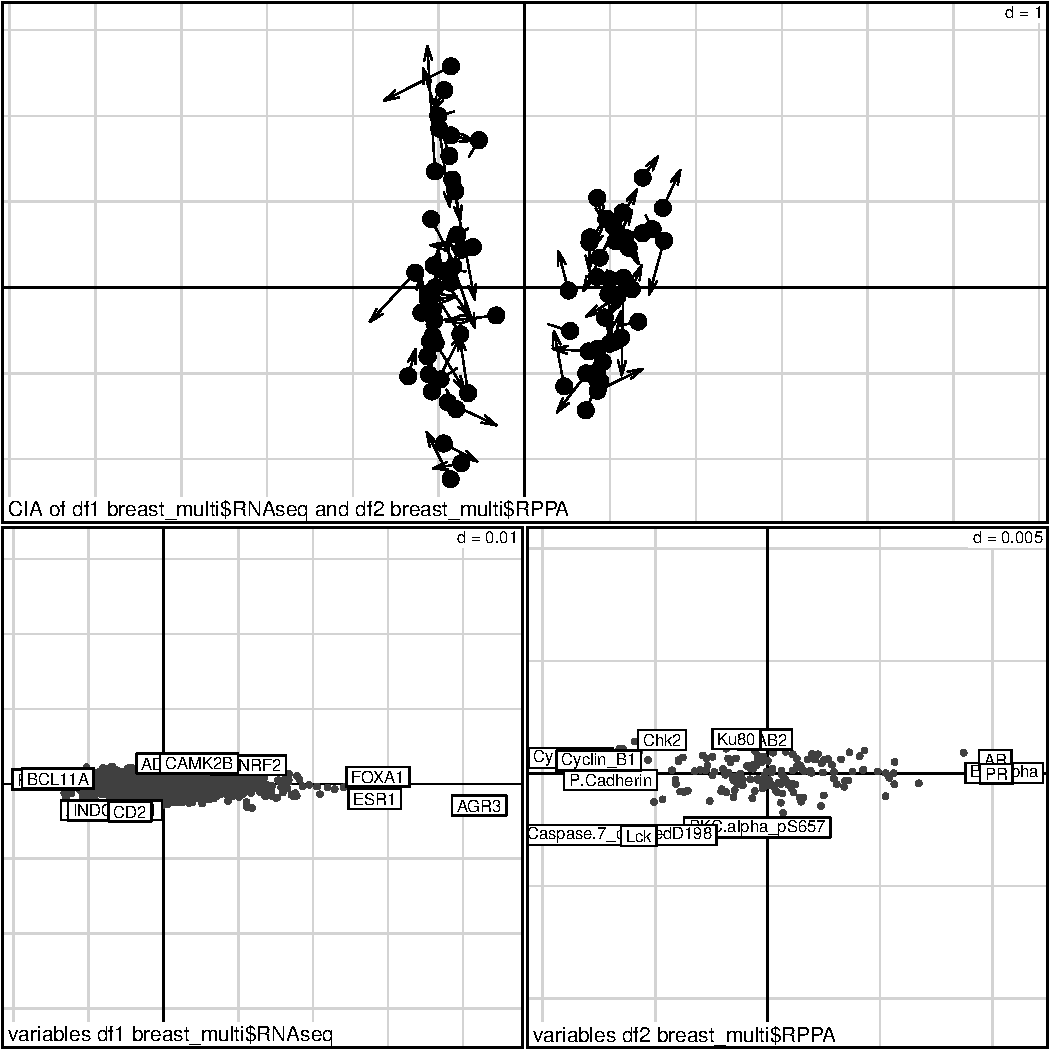
\includegraphics[width=6cm]{figure/plot_cia-1}
\end{center}
\end{figure}

\end{frame}


\begin{frame}[fragile, plain]\frametitle{Co-inertia: gene expression and proteins}

Top-5 features of the first axis (positive side) can be retrieve by

\footnotesize
\begin{knitrout}\footnotesize
\definecolor{shadecolor}{rgb}{0.969, 0.969, 0.969}\color{fgcolor}\begin{kframe}
\begin{alltt}
\hlkwd{topVar}\hlstd{(resCIA,} \hlkwc{axis}\hlstd{=}\hlnum{1}\hlstd{,} \hlkwc{topN}\hlstd{=}\hlnum{5}\hlstd{,} \hlkwc{end}\hlstd{=}\hlstr{"positive"}\hlstd{)}
\end{alltt}
\begin{verbatim}
##   ax1_df1_positive ax1_df2_positive
## 1             AGR3         ER.alpha
## 2            FOXA1               PR
## 3             ESR1               AR
## 4             AGR2           INPP4B
## 5          C1orf64            GATA3
\end{verbatim}
\end{kframe}
\end{knitrout}

\end{frame}



\begin{frame}[fragile, plain]\frametitle{Co-inertia: gene expression and proteins}

Top-5 features of the first axis (negative side) can be retrieve by

\footnotesize
\begin{knitrout}\footnotesize
\definecolor{shadecolor}{rgb}{0.969, 0.969, 0.969}\color{fgcolor}\begin{kframe}
\begin{alltt}
\hlkwd{topVar}\hlstd{(resCIA,} \hlkwc{axis}\hlstd{=}\hlnum{1}\hlstd{,} \hlkwc{topN}\hlstd{=}\hlnum{5}\hlstd{,} \hlkwc{end}\hlstd{=}\hlstr{"negative"}\hlstd{)}
\end{alltt}
\begin{verbatim}
##   ax1_df1_negative      ax1_df2_negative
## 1            ROPN1             Cyclin_E1
## 2           ROPN1B             Cyclin_B1
## 3           BCL11A            P.Cadherin
## 4             ART3                  MSH6
## 5            SFRP1 Caspase.7_cleavedD198
\end{verbatim}
\end{kframe}
\end{knitrout}

\end{frame}



\begin{frame}[fragile, plain]\frametitle{More than two tables}


\begin{knitrout}\footnotesize
\definecolor{shadecolor}{rgb}{0.969, 0.969, 0.969}\color{fgcolor}\begin{kframe}
\begin{alltt}
\hlstd{resMCIA} \hlkwb{<-} \hlkwd{mcia}\hlstd{( breast_multi[} \hlkwd{c}\hlstd{(}\hlnum{1}\hlstd{,}\hlnum{3}\hlstd{,}\hlnum{4}\hlstd{,}\hlnum{5}\hlstd{,}\hlnum{6}\hlstd{,}\hlnum{7}\hlstd{) ] )}
\end{alltt}
\end{kframe}
\end{knitrout}


\begin{knitrout}\footnotesize
\definecolor{shadecolor}{rgb}{0.969, 0.969, 0.969}\color{fgcolor}\begin{kframe}
\begin{alltt}
\hlkwd{plot}\hlstd{(resMCIA,} \hlkwc{axes}\hlstd{=}\hlnum{1}\hlopt{:}\hlnum{2}\hlstd{,} \hlkwc{sample.lab}\hlstd{=}\hlnum{FALSE}\hlstd{,} \hlkwc{sample.legend}\hlstd{=}\hlnum{FALSE}\hlstd{,}
     \hlkwc{phenovec}\hlstd{=group,} \hlkwc{gene.nlab}\hlstd{=}\hlnum{2}\hlstd{,}
     \hlkwc{df.color}\hlstd{=}\hlkwd{c}\hlstd{(}\hlstr{"cyan"}\hlstd{,} \hlstr{"magenta"}\hlstd{,} \hlstr{"red4"}\hlstd{,} \hlstr{"brown"}\hlstd{,}\hlstr{"yellow"}\hlstd{,} \hlstr{"orange"}\hlstd{),}
     \hlkwc{df.pch}\hlstd{=}\hlnum{2}\hlopt{:}\hlnum{7}\hlstd{)}
\end{alltt}
\end{kframe}
\end{knitrout}
\end{frame}


\begin{frame}[fragile, plain]\frametitle{More than two tables}

\begin{figure}
\begin{center}
 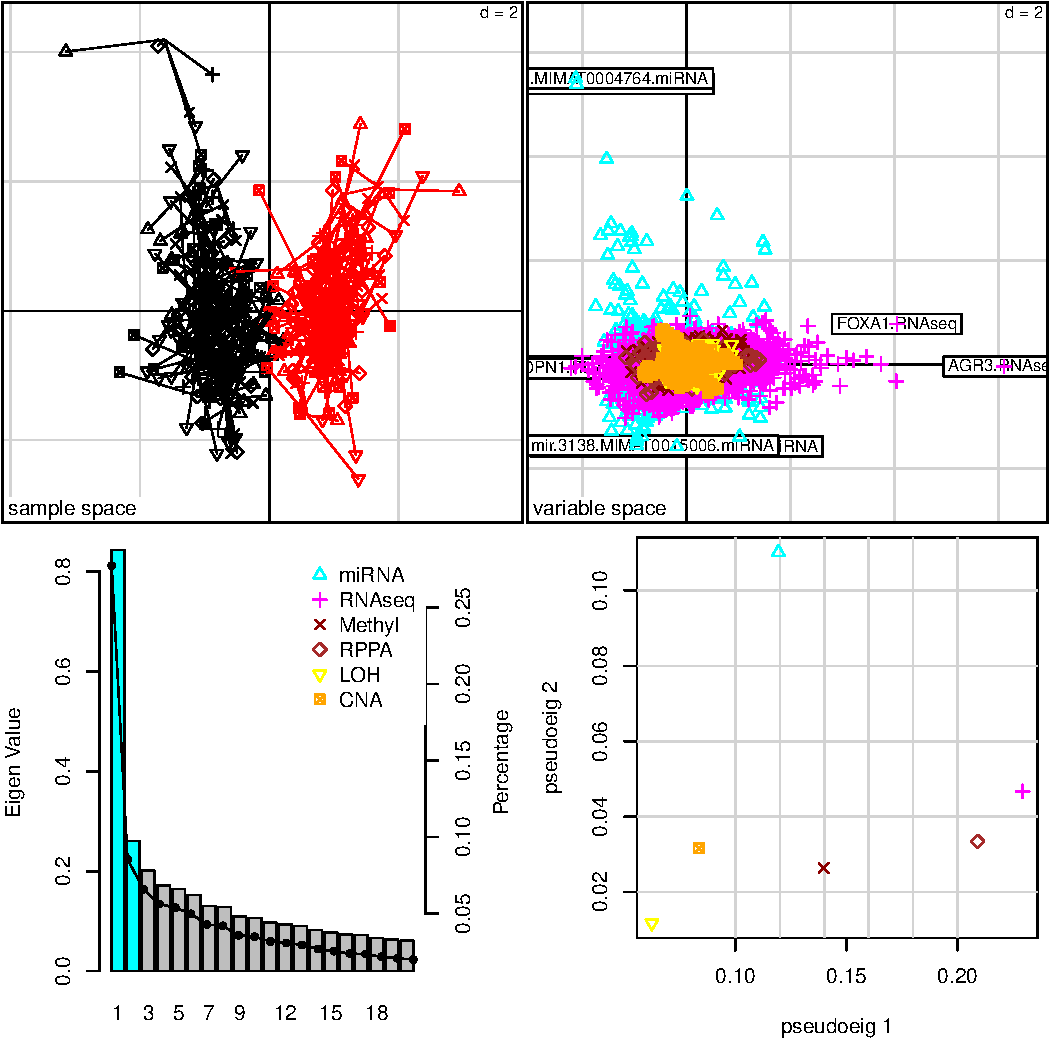
\includegraphics[width=5.5cm]{figure/plot_mcia-1}
\end{center}
\end{figure}

\end{frame}

\begin{frame}[fragile, plain]\frametitle{More than two tables}

Top-5 features of the first axis (positive side) can be retrieve by

\scriptsize
\begin{knitrout}\footnotesize
\definecolor{shadecolor}{rgb}{0.969, 0.969, 0.969}\color{fgcolor}\begin{kframe}
\begin{alltt}
\hlkwd{topVar}\hlstd{(resMCIA,} \hlkwc{end}\hlstd{=}\hlstr{"positive"}\hlstd{,} \hlkwc{axis}\hlstd{=}\hlnum{1}\hlstd{,} \hlkwc{topN}\hlstd{=}\hlnum{5}\hlstd{)}
\end{alltt}
\begin{verbatim}
##                ax1_miRNA_positive ax1_RNAseq_positive ax1_Methyl_positive
## 1 hsa.mir.4254.MIMAT0016884.miRNA         AGR3.RNAseq   cg08097882.Methyl
## 2 hsa.mir.3945.MIMAT0018361.miRNA        FOXA1.RNAseq   cg09952204.Methyl
## 3 hsa.mir.302b.MIMAT0000715.miRNA         ESR1.RNAseq   cg04988423.Methyl
## 4 hsa.mir.1265.MIMAT0005918.miRNA         AGR2.RNAseq   cg00679738.Methyl
## 5 hsa.mir.3171.MIMAT0015046.miRNA      C1orf64.RNAseq   cg12601757.Methyl
##   ax1_RPPA_positive ax1_LOH_positive ax1_CNA_positive
## 1     ER.alpha.RPPA        X4006.LOH        X8374.CNA
## 2           AR.RPPA        X4007.LOH        X8381.CNA
## 3           PR.RPPA        X4008.LOH        X8382.CNA
## 4       INPP4B.RPPA        X4009.LOH        X8383.CNA
## 5        GATA3.RPPA        X4010.LOH        X8384.CNA
\end{verbatim}
\end{kframe}
\end{knitrout}

\end{frame}



\begin{frame}[fragile, plain]\frametitle{More than two tables}

\begin{knitrout}\footnotesize
\definecolor{shadecolor}{rgb}{0.969, 0.969, 0.969}\color{fgcolor}\begin{kframe}
\begin{alltt}
\hlkwd{plot}\hlstd{(resMCIA}\hlopt{$}\hlstd{mcoa}\hlopt{$}\hlstd{cov2,}  \hlkwc{xlab} \hlstd{=} \hlstr{"pseudoeig 1"}\hlstd{,}
     \hlkwc{ylab} \hlstd{=} \hlstr{"pseudoeig 2"}\hlstd{,} \hlkwc{pch}\hlstd{=}\hlnum{19}\hlstd{,} \hlkwc{col}\hlstd{=}\hlstr{"red"}\hlstd{)}
\hlkwd{text}\hlstd{(resMCIA}\hlopt{$}\hlstd{mcoa}\hlopt{$}\hlstd{cov2,} \hlkwc{labels}\hlstd{=}\hlkwd{rownames}\hlstd{(resMCIA}\hlopt{$}\hlstd{mcoa}\hlopt{$}\hlstd{cov2),}
     \hlkwc{cex}\hlstd{=}\hlnum{1.4}\hlstd{,} \hlkwc{adj}\hlstd{=}\hlnum{0}\hlstd{)}
\end{alltt}
\end{kframe}
\end{knitrout}

\begin{figure}
\begin{center}
 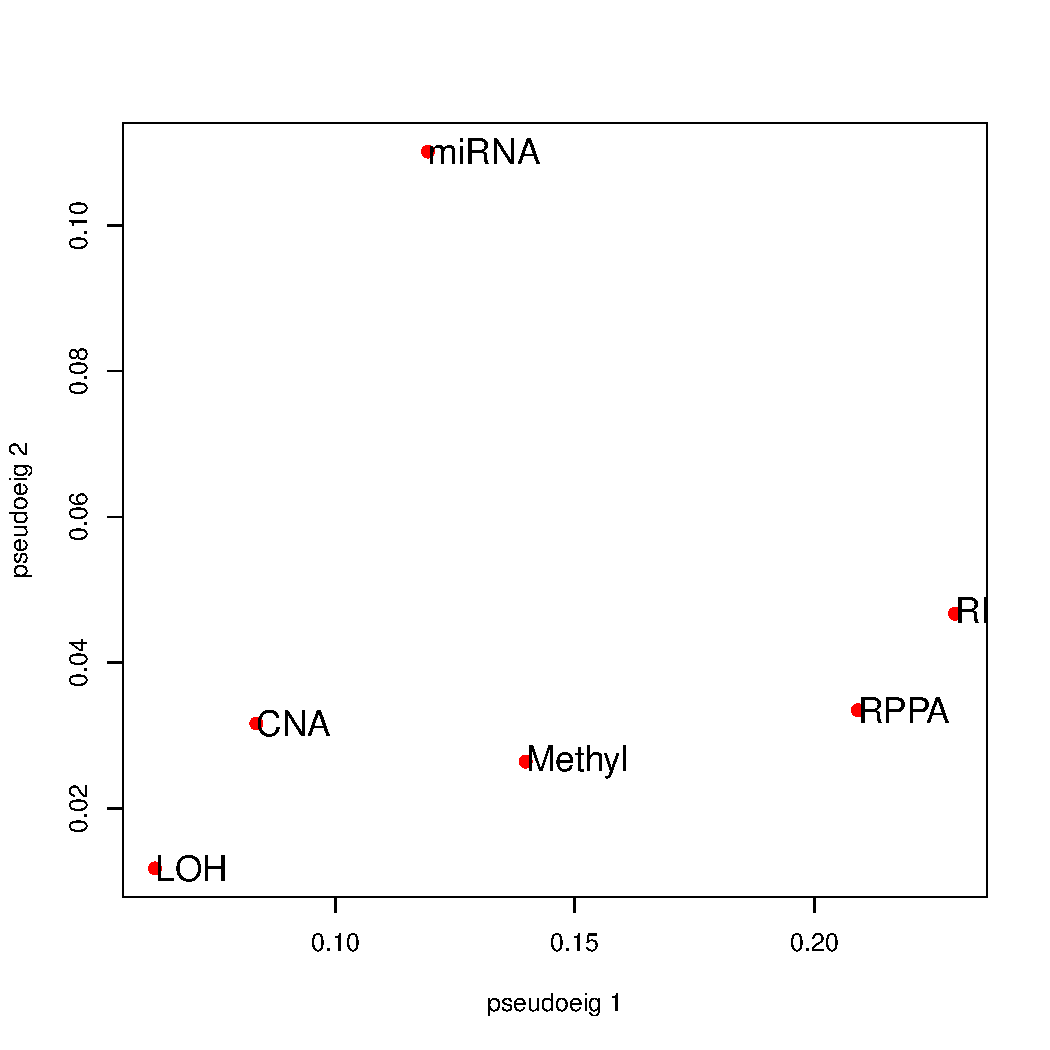
\includegraphics[width=5.5cm]{figure/plot_eigen-1}
\end{center}
\end{figure}

\end{frame}


%%%%%%%%%%%%%%%%%%%%%%%%%%%%%%%%%%%
\section{RGCCA}
%%%%%%%%%%%%%%%%%%%%%%%%%%%%%%%%%%%


\begin{frame}[plain]\frametitle{RGCCA}

\begin{itemize}
 \item RGCCA allows to combine tables with different types of variables between blocks
 \item The objective of RGCCA is to find, for each block (talbe), a weighted composite of variables (called block component) $\y_j= \X_j \ma a_j,j=1, \ldots,J$ (where $\ma a_j$ is a column-vector with  $p_j$ elements) summarizing the relevant information between and within the blocks. 
 \item The block components are obtained such that (i) block components explain well their own block and/or (ii) block components that are assumed to be connected are highly correlated. 
 \item RGCCA has been extended to integrate a variable selection procedure, called SGCCA, allowing the identification of the most relevant features.
\end{itemize}

\end{frame}


\begin{frame}[plain]\frametitle{RGCCA}

RGCCA (Tenenhaus, M. et al. Psychometrika, 2001 and Tenenhaus A et al, Psychometrika, 2017) is defined as the next optimization problem:

\begin{equation*}
\displaystyle \underset{\ma a_1,\ma a_2, \ldots,\ma a_J}{\text{maximize}} \sum_{j, k = 1}^J c_{jk}g(\mathrm{cov}(\X_j\ma a_j, \X_k\ma a_k)) \\ \mathrm{~~s.t.~~} (1-\tau_j)\mathrm{var}(\X_j\ma a_j) + \tau_j\Vert \ma a_j \Vert^2 = 1, j=1, \ldots,J
\end{equation*}

\end{frame}


\begin{frame}[plain]\frametitle{RGCCA}

\begin{itemize}
 \item The scheme function $g$ is any continuous convex function and allows to consider different optimization criteria.  
  \begin{itemize}
   \item identity (horst scheme, leading to maximizing the sum of covariances between block components)
   \item the absolute value (centroid scheme, yielding maximization of the sum of the absolute values of the covariances)
   \item the square function (factorial scheme, thereby maximizing the sum of squared covariances)
   \item any even integer $m$, $g(x) = x^m$  
  \end{itemize} 
  \item A fair model is a model where all blocks contribute equally to the solution ($m=1$)
  \item $m>1$ is preferable if the user wants to discriminate between blocks. 
  \item In practice, $m$ is equal to $1$, $2$ or $4$. The higher the value of $m$ the more the method acts as block selector
\end{itemize}

\end{frame}


\begin{frame}[plain]\frametitle{RGCCA}

The design matrix $\ma C$ is a symmetric  $J \times J$ matrix of nonnegative elements describing the network of connections between blocks that the user wants to take into account. Usually, $c_{jk}=1$ for two connected blocks and 0 otherwise.

\end{frame}

\begin{frame}[plain]\frametitle{RGCCA}


\begin{figure}
\begin{center}
 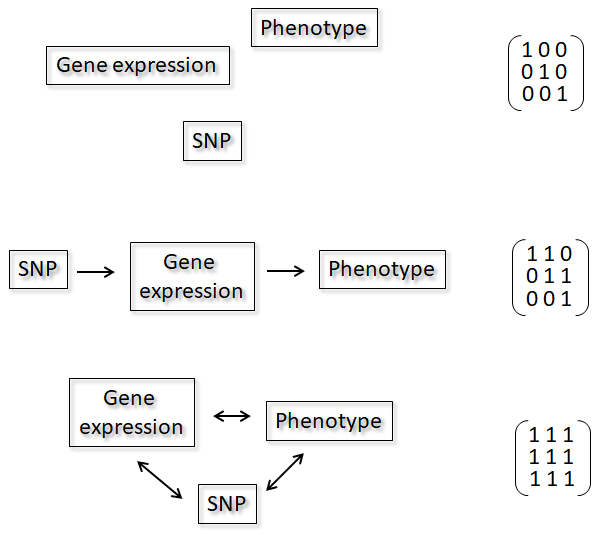
\includegraphics[height=6cm, width=6.5cm]{figures/rgcca.png}
\end{center}
\end{figure}
\end{frame}


\begin{frame}[plain]\frametitle{RGCCA}

The $\tau_j$  are called shrinkage parameters ranging from $0$ to $1$ and interpolate smoothly between maximizing the covariance and maximizing the correlation

\begin{itemize}
 \item $\tau_j=1$ yields the maximization of a covariance-based criterion. It is recommended when the user wants a stable component (large variance) while simultaneously taking into account the correlations 
between blocks. The user must, however, be aware that variance dominates over correlation.
    \item $\tau_j=0$ yields the maximization of a correlation-based criterion. It is recommended when the user wants to maximize correlations between connected components. This option can yield unstable solutions in case of multi-collinearity and cannot be used when a data block is rank deficient (e.g. $n<p_j$).
    \item $0<\tau_j<1$ is a good compromise between variance and correlation: the block components are simultaneously stable and as well correlated as possible with their connected block components. This setting can be used when the data block is rank deficient. 

\end{itemize}

\end{frame}



\begin{frame}[fragile, plain]\frametitle{PCA as RGCCA}

Principal Component Analysis is defined as the following optimization problem 

\begin{equation*}
\underset{\ma a}{\text{maximize}} \text{~~var}\left(\X \ma a \right) \mathrm{~s.t.~} \Vert \ma a \Vert = 1
\label{PCA1}
\end{equation*}

and is obtained with the `rgcca()` function as follows:

\begin{knitrout}\footnotesize
\definecolor{shadecolor}{rgb}{0.969, 0.969, 0.969}\color{fgcolor}\begin{kframe}
\begin{alltt}
\hlcom{# Design matrix C}
\hlcom{# Shrinkage parameters tau = c(tau1, tau2)}

\hlstd{pca.with.rgcca} \hlkwb{=} \hlkwd{rgcca}\hlstd{(}\hlkwc{A} \hlstd{=} \hlkwd{list}\hlstd{(X, X),}
                       \hlkwc{C} \hlstd{=} \hlkwd{matrix}\hlstd{(}\hlkwd{c}\hlstd{(}\hlnum{0}\hlstd{,} \hlnum{1}\hlstd{,} \hlnum{1}\hlstd{,} \hlnum{0}\hlstd{),} \hlnum{2}\hlstd{,} \hlnum{2}\hlstd{),}
                       \hlkwc{tau} \hlstd{=} \hlkwd{c}\hlstd{(}\hlnum{1}\hlstd{,} \hlnum{1}\hlstd{))}
\end{alltt}
\end{kframe}
\end{knitrout}
\end{frame}


\begin{frame}[fragile, plain]\frametitle{CCA as RGCCA}

Canonical Correlation Analysis is defined as the following optimization problem 

\begin{equation*}
\underset{\ma a_1, \ma a_2}{\text{maximize}} \text{
~~cor}\left(\X_1\ma a_1, \X_2\ma a_2 \right) \mathrm{~s.t.~} \text{var}(\X_1\ma a_1) = \text{var}(\X_2\ma a_2) = 1
\label{CCA}
\end{equation*}

and is obtained with the `rgcca()` function as follows:


\begin{knitrout}\footnotesize
\definecolor{shadecolor}{rgb}{0.969, 0.969, 0.969}\color{fgcolor}\begin{kframe}
\begin{alltt}
\hlcom{# X1 = Block1 and X2 = Block2 }
\hlcom{# Design matrix C}
\hlcom{# Shrinkage parameters tau = c(tau1, tau2)}

\hlstd{cca.with.rgcca} \hlkwb{=} \hlkwd{rgcca}\hlstd{(}\hlkwc{A}\hlstd{=} \hlkwd{list}\hlstd{(X1, X2),}
                       \hlkwc{C} \hlstd{=} \hlkwd{matrix}\hlstd{(}\hlkwd{c}\hlstd{(}\hlnum{0}\hlstd{,} \hlnum{1}\hlstd{,} \hlnum{1}\hlstd{,} \hlnum{0}\hlstd{),} \hlnum{2}\hlstd{,} \hlnum{2}\hlstd{),}
                       \hlkwc{tau} \hlstd{=} \hlkwd{c}\hlstd{(}\hlnum{0}\hlstd{,} \hlnum{0}\hlstd{))}
\end{alltt}
\end{kframe}
\end{knitrout}

\end{frame}




\begin{frame}[fragile, plain]\frametitle{PLS as RGCCA}
PLS regression is defined as the following optimization problem 

\begin{equation*}
\underset{\ma a_1, \ma a_2}{\text{maximize}} \text{
~~cov}\left(\X_1\ma a_1, \X_2\ma a_2 \right) \mathrm{~s.t.~} \Vert \ma a_1 \Vert = \Vert \ma a_2 \Vert = 1
\label{PLS}
\end{equation*}

and is obtained with the `rgcca()` function as follows:


\begin{knitrout}\footnotesize
\definecolor{shadecolor}{rgb}{0.969, 0.969, 0.969}\color{fgcolor}\begin{kframe}
\begin{alltt}
\hlcom{# X1 = Block1 and X2 = Block2 }
\hlcom{# Design matrix C}
\hlcom{# Shrinkage parameters tau = c(tau1, tau2)}

\hlstd{pls.with.rgcca} \hlkwb{=} \hlkwd{rgcca}\hlstd{(}\hlkwc{A}\hlstd{=} \hlkwd{list}\hlstd{(X1, X2),}
                       \hlkwc{C} \hlstd{=} \hlkwd{matrix}\hlstd{(}\hlkwd{c}\hlstd{(}\hlnum{0}\hlstd{,} \hlnum{1}\hlstd{,} \hlnum{1}\hlstd{,} \hlnum{0}\hlstd{),} \hlnum{2}\hlstd{,} \hlnum{2}\hlstd{),}
                       \hlkwc{tau} \hlstd{=} \hlkwd{c}\hlstd{(}\hlnum{1}\hlstd{,} \hlnum{1}\hlstd{))}
\end{alltt}
\end{kframe}
\end{knitrout}


\end{frame}



\begin{frame}[fragile, plain]\frametitle{RDA as RGCCA}

Redundancy Analysis of $\X_1$ with respect to $\X_2$ is defined as the following optimization problem 

\begin{equation*}
\underset{\ma a_1, \ma a_2}{\text{maximize}} \text{
~~cor}\left(\X_1 \ma a_1, \X_2 \ma a_2 \right) \times \text{
var}\left(\X_1\ma a_1\right)^{1/2} \mathrm{~s.t.~} \Vert \ma a_1 \Vert = \text{var}(\X_2\ma a_2) = 1
\label{RA}
\end{equation*}

and is obtained with the `rgcca()` function as follows:

\begin{knitrout}\footnotesize
\definecolor{shadecolor}{rgb}{0.969, 0.969, 0.969}\color{fgcolor}\begin{kframe}
\begin{alltt}
\hlcom{# X1 = Block1 and X2 = Block2 }
\hlcom{# Design matrix C}
\hlcom{# Shrinkage parameters tau = c(tau1, tau2)}

\hlstd{ra.with.rgcca} \hlkwb{=} \hlkwd{rgcca}\hlstd{(}\hlkwc{A}\hlstd{=} \hlkwd{list}\hlstd{(X1, X2),}
                       \hlkwc{C} \hlstd{=} \hlkwd{matrix}\hlstd{(}\hlkwd{c}\hlstd{(}\hlnum{0}\hlstd{,} \hlnum{1}\hlstd{,} \hlnum{1}\hlstd{,} \hlnum{0}\hlstd{),} \hlnum{2}\hlstd{,} \hlnum{2}\hlstd{),}
                       \hlkwc{tau} \hlstd{=} \hlkwd{c}\hlstd{(}\hlnum{1}\hlstd{,} \hlnum{0}\hlstd{))}
\end{alltt}
\end{kframe}
\end{knitrout}
\end{frame}

\begin{frame}[fragile, plain]\frametitle{GCCA as RGCCA}

For Generalized Canonical Correlation Analysis (GCCA), a superblock $\ma X_{J+1} = \left[\ma X_1, \dots, \ma X_J \right]$ defined as the concatenation of all the blocks is introduced. GCCA is defined as the following optimization problem 

\begin{equation*}
\underset{\ma a_1, \ma a_2, \ldots,\ma a_J} {\text{maximize}} \displaystyle \sum_{j=1}^J \text{cor}^2(\ma X_j\ma a_j, \ma X_{J+1}\ma a_{J+1}) \text{~~s.t~~} \text{var}(\X_j \ma a_j) = 1, j=1, \ldots, J+1
\end{equation*}

and is obtained with the `rgcca()` function as follows:
\begin{knitrout}\footnotesize
\definecolor{shadecolor}{rgb}{0.969, 0.969, 0.969}\color{fgcolor}\begin{kframe}
\begin{alltt}
\hlcom{# X1 = Block1, ..., XJ = BlockJ, X_\{J+1\} = [X1, ..., XJ]}
\hlcom{# (J+1)*(J+1) Design matrix C}
C = \hlkwd{matrix}(\hlkwd{c}(0, 0, 0, ..., 0, 1,
             0, 0, 0, ..., 0, 1,
                    ...
             1, 1, 1, ..., 1, 0), J+1, J+1)
\hlcom{# Shrinkage parameters tau = c(tau1, ...,  tauJ, tau_\{J+1\})}
gcca.with.rgcca = \hlkwd{rgcca}(A= \hlkwd{list}(X1, ..., XJ, \hlkwd{cbind}(X1, ..., XJ)), 
                       C = C, tau = \hlkwd{rep}(0, J+1),
                       scheme = \hlstr{"factorial"})
\end{alltt}
\end{kframe}
\end{knitrout}
\end{frame}


\begin{frame}[fragile, plain]\frametitle{MCIA as RGCCA}

For Multiple Co-Inertia Analysis (MCIA) a superblock $\ma X_{J+1} = [\ma X_1, \dots, \ma X_J$ defined as the concatenation of all the blocks is introduced. MCIA is defined as the following optimization problem 

\begin{equation}
\underset{\ma a_1, \ma a_2, \ldots,\ma a_J} {\text{maximize}} \displaystyle \sum_{j=1}^J \text{cor}^2(\ma X_j\ma a_j, \ma X_{J+1}\ma a_{J+1})\times \text{var}(\X_j\ma a_j), \text{~~s.t~~} \Vert \ma a_j \Vert = 1, j=1, \ldots, J \text{~~and~~} \text{var}(\X_{J+1}\ma a_{J+1}) = 1
\end{equation}

and is obtained with the `rgcca()` function as follows:
\begin{knitrout}\footnotesize
\definecolor{shadecolor}{rgb}{0.969, 0.969, 0.969}\color{fgcolor}\begin{kframe}
\begin{alltt}
\hlcom{# X1 = Block1, ..., XJ = BlockJ, X_\{J+1\} = [X1, ..., XJ]}
\hlcom{# (J+1)*(J+1) Design matrix C}
C = \hlkwd{matrix}(\hlkwd{c}(0, 0, 0, ..., 0, 1,
             0, 0, 0, ..., 0, 1,
                  ...
             1, 1, 1, ..., 1, 0), J+1, J+1)
\hlcom{# Shrinkage parameters tau = c(tau1, ...,  tauJ, tau_\{J+1\})}
mcoa.with.rgcca = \hlkwd{rgcca}(A= \hlkwd{list}(X1, ..., XJ, \hlkwd{cbind}(X1, ..., XJ)), 
                       C = C, tau = \hlkwd{c}(\hlkwd{rep}(1, J), 0),
                       scheme = \hlstr{"factorial"})
\end{alltt}
\end{kframe}
\end{knitrout}
\end{frame}




\begin{frame}[fragile, plain]\frametitle{RGCCA data analysis}

Data must be preprocessed to ensure comparability between variables.  Standardization is applied (zero mean and unit variance). 

\begin{knitrout}\footnotesize
\definecolor{shadecolor}{rgb}{0.969, 0.969, 0.969}\color{fgcolor}\begin{kframe}
\begin{alltt}
\hlkwd{library}\hlstd{(RGCCA)}
\hlkwd{load}\hlstd{(}\hlstr{"data/breast_TCGA.RData"}\hlstd{)}
\hlstd{X} \hlkwb{<-} \hlkwd{t}\hlstd{(breast_multi}\hlopt{$}\hlstd{RNAseq)}
\hlstd{Y} \hlkwb{<-} \hlkwd{t}\hlstd{(breast_multi}\hlopt{$}\hlstd{miRNA)}
\hlstd{Z} \hlkwb{<-} \hlkwd{t}\hlstd{(breast_multi}\hlopt{$}\hlstd{RPPA)}
\hlstd{A} \hlkwb{<-} \hlkwd{list}\hlstd{(}\hlkwc{rnaseq}\hlstd{=X,} \hlkwc{miRNA}\hlstd{=Y,} \hlkwc{RPPA}\hlstd{=Z)}
\hlstd{A} \hlkwb{<-} \hlkwd{lapply}\hlstd{(A, scale)}
\end{alltt}
\end{kframe}
\end{knitrout}

NOTE: A possible strategy is to standardize the variables and then to divide each block by the square root of its number of variables. This two-step procedure leads to $\mathrm{tr}(\ma X_j^t \ma X_j )=n$  for each block (i.e. the sum of the eigenvalues of the covariance matrix of $\ma X_j$ is equal to $1$ whatever the block). Such a preprocessing is reached by setting the `scale` argument to `TRUE` (default value) in the `rgcca()` and `sgcca()` functions.



\end{frame}


\begin{frame}[fragile, plain]\frametitle{RGCCA data analysis}

Let us assume that both miRNA and mRNa are affecting the protein levels. Therefore the $\ma C$ matrix will be

\begin{knitrout}\footnotesize
\definecolor{shadecolor}{rgb}{0.969, 0.969, 0.969}\color{fgcolor}\begin{kframe}
\begin{alltt}
\hlstd{C} \hlkwb{<-} \hlkwd{matrix}\hlstd{(}\hlkwd{c}\hlstd{(}\hlnum{1}\hlstd{,}\hlnum{0}\hlstd{,}\hlnum{1}\hlstd{,}\hlnum{0}\hlstd{,}\hlnum{1}\hlstd{,}\hlnum{1}\hlstd{,}\hlnum{0}\hlstd{,}\hlnum{0}\hlstd{,}\hlnum{1}\hlstd{),} \hlkwc{nrow}\hlstd{=}\hlnum{3}\hlstd{,} \hlkwc{byrow} \hlstd{=} \hlnum{TRUE}\hlstd{)}
\hlstd{C}
\end{alltt}
\begin{verbatim}
##      [,1] [,2] [,3]
## [1,]    1    0    1
## [2,]    0    1    1
## [3,]    0    0    1
\end{verbatim}
\end{kframe}
\end{knitrout}

\end{frame}


\begin{frame}[fragile, plain]\frametitle{RGCCA data analysis}

RGCCA using the defined design matrix $\ma C$, the factorial scheme ($g(x) = x^2$) and mode B for all blocks (full correlation criterion) is obtained by

\begin{knitrout}\footnotesize
\definecolor{shadecolor}{rgb}{0.969, 0.969, 0.969}\color{fgcolor}\begin{kframe}
\begin{alltt}
\hlstd{rgcca.factorial} \hlkwb{<-} \hlkwd{rgcca}\hlstd{(A,} \hlkwc{C}\hlstd{=C,} \hlkwc{tau} \hlstd{=} \hlkwd{rep}\hlstd{(}\hlnum{0}\hlstd{,} \hlnum{3}\hlstd{),}
                           \hlkwc{scheme} \hlstd{=}\hlstr{"factorial"}\hlstd{,} \hlkwc{ncomp}\hlstd{=}\hlkwd{c}\hlstd{(}\hlnum{2}\hlstd{,}\hlnum{2}\hlstd{,}\hlnum{2}\hlstd{),}
                           \hlkwc{scale} \hlstd{=} \hlnum{FALSE}\hlstd{,} \hlkwc{verbose} \hlstd{=} \hlnum{FALSE}\hlstd{)}
\end{alltt}
\end{kframe}
\end{knitrout}

The weight vectors, solution of the optimization problemare obtained as:

\begin{knitrout}\footnotesize
\definecolor{shadecolor}{rgb}{0.969, 0.969, 0.969}\color{fgcolor}\begin{kframe}
\begin{alltt}
\hlstd{rgcca.factorial}\hlopt{$}\hlstd{a} \hlcom{# weight vectors}
\end{alltt}
\end{kframe}
\end{knitrout}

\end{frame}


\begin{frame}[fragile, plain]\frametitle{RGCCA data analysis}

The block-components are also avalaible as output of `rgcca`. The first components of each block are given by:

\begin{knitrout}\footnotesize
\definecolor{shadecolor}{rgb}{0.969, 0.969, 0.969}\color{fgcolor}\begin{kframe}
\begin{alltt}
\hlstd{Y.block} \hlkwb{<-} \hlstd{rgcca.factorial}\hlopt{$}\hlstd{Y}
\hlkwd{lapply}\hlstd{(Y.block, head)}
\end{alltt}
\begin{verbatim}
## [[1]]
##                   comp1      comp2
## TCGA-C8-A12V -1.4043762 -0.5590542
## TCGA-A2-A0ST -1.3471553 -2.3964964
## TCGA-E2-A159 -0.5738528  0.8281707
## TCGA-BH-A0BW -0.2061025  0.4681924
## TCGA-A2-A0SX -0.8960506  0.1448149
## TCGA-AR-A1AI -1.2582255  0.4333885
## 
## [[2]]
##                   comp1      comp2
## TCGA-C8-A12V -1.4043119 -0.5584358
## TCGA-A2-A0ST -1.3470213 -2.3960350
## TCGA-E2-A159 -0.5738116  0.8287364
## TCGA-BH-A0BW -0.2062718  0.4694125
## TCGA-A2-A0SX -0.8958721  0.1451569
## TCGA-AR-A1AI -1.2582603  0.4338262
## 
## [[3]]
##                   comp1      comp2
## TCGA-C8-A12V -1.4044965  0.5580687
## TCGA-A2-A0ST -1.3472866  2.3958390
## TCGA-E2-A159 -0.5738029 -0.8288787
## TCGA-BH-A0BW -0.2059072 -0.4690433
## TCGA-A2-A0SX -0.8960716 -0.1455184
## TCGA-AR-A1AI -1.2581428 -0.4338783
\end{verbatim}
\end{kframe}
\end{knitrout}
\end{frame}



\begin{frame}[fragile, plain]\frametitle{RGCCA data analysis}

Information about Average Variance Explained (AVE)

- The AVE of block $\ma X_j$, denoted by AVE($\ma X_j$), is defined as:

\begin{equation*}
\mathrm{AVE}(\ma X_j)=  1/p_j \sum_{h=1}^{p_j} cor^2( \ma x_{jh},\ma y_j)
\end{equation*}

AVE($\ma X_j$) varies between 0 and 1 and reflects the proportion of variance captured by $\ma y_j$.

- For all blocks:

\begin{equation*}
\displaystyle \mathrm{AVE(outer model)} = \left( 1/\sum_j p_j \right) \sum_j p_j \mathrm{AVE}(\ma X_j)
\end{equation*}

- For the inner model:

\begin{equation*}
\displaystyle \mathrm{AVE(inner model)} = \left( 1/\sum_{j<k} c_{jk} \right) \sum_{j<k} c_{jk} \mathrm{cor}^2(\ma y_j , \ma y_k)
\end{equation*}

\end{frame}


\begin{frame}[fragile, plain]\frametitle{RGCCA data analysis}

\begin{knitrout}\footnotesize
\definecolor{shadecolor}{rgb}{0.969, 0.969, 0.969}\color{fgcolor}\begin{kframe}
\begin{alltt}
\hlstd{rgcca.factorial}\hlopt{$}\hlstd{AVE}
\end{alltt}
\begin{verbatim}
## $AVE_X
## $AVE_X[[1]]
##     comp1     comp2 
## 0.1470807 0.0303539 
## 
## $AVE_X[[2]]
##      comp1      comp2 
## 0.06683530 0.02441686 
## 
## $AVE_X[[3]]
##      comp1      comp2 
## 0.17983101 0.07924063 
## 
## 
## $AVE_outer_model
## [1] 0.14088037 0.03060966
## 
## $AVE_inner_model
## [1] 1 1
\end{verbatim}
\end{kframe}
\end{knitrout}

\end{frame}


\begin{frame}[fragile, plain]\frametitle{RGCCA data analysis}

Plot individuals

\begin{knitrout}\footnotesize
\definecolor{shadecolor}{rgb}{0.969, 0.969, 0.969}\color{fgcolor}\begin{kframe}
\begin{alltt}
\hlkwd{source}\hlstd{(}\hlstr{"R/plotInd.R"}\hlstd{)}
\hlkwd{plotInd}\hlstd{(rgcca.factorial, group)}
\end{alltt}
\end{kframe}
\end{knitrout}
\end{frame}  



\begin{frame}[fragile, plain]\frametitle{RGCCA data analysis}

\begin{figure}
\begin{center}
 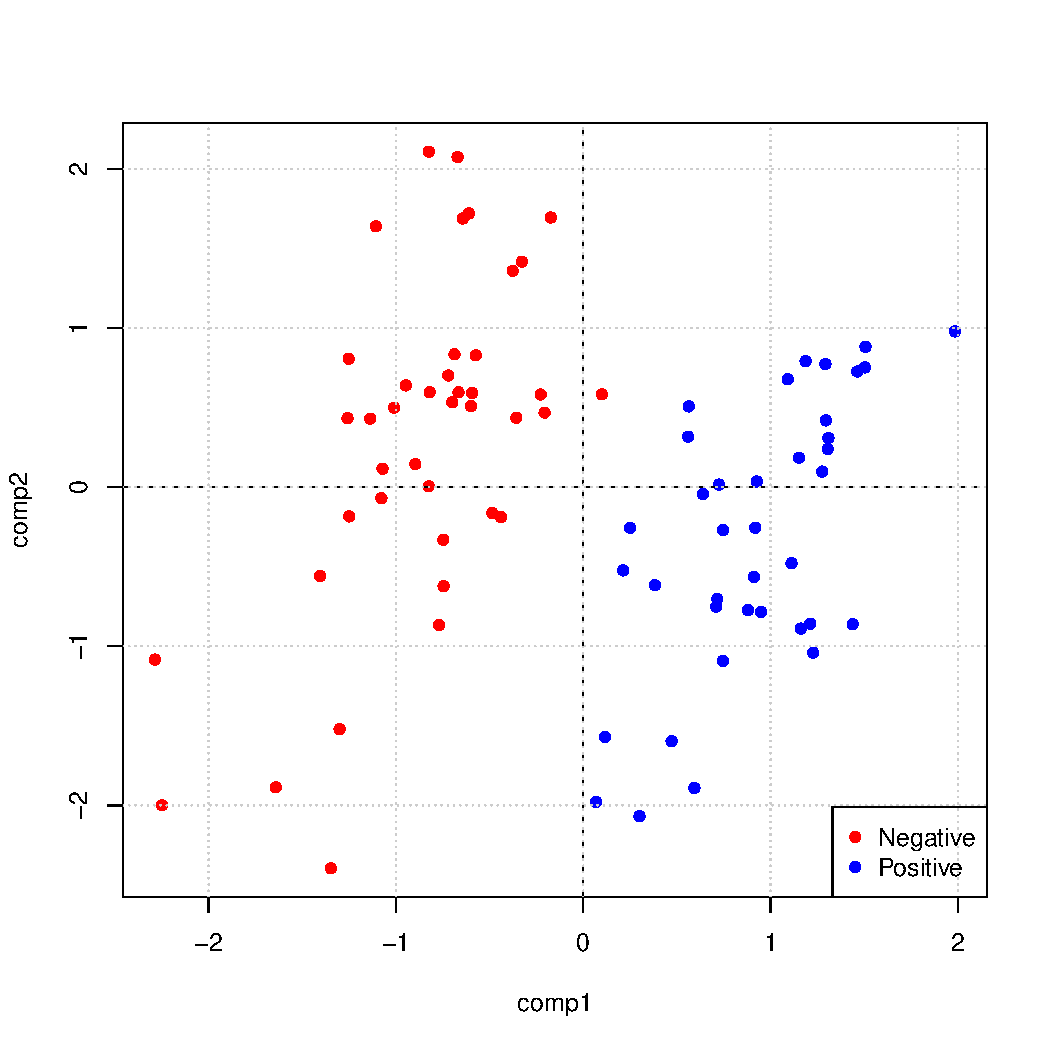
\includegraphics[width=5.5cm]{figure/rgcca_ind-1}
\end{center}
\end{figure}

\end{frame}


\begin{frame}[fragile, plain]\frametitle{RGCCA data analysis}

Features first axis right side (e.g. ER+)

\begin{knitrout}\footnotesize
\definecolor{shadecolor}{rgb}{0.969, 0.969, 0.969}\color{fgcolor}\begin{kframe}
\begin{alltt}
\hlkwd{source}\hlstd{(}\hlstr{"R/topVars.R"}\hlstd{)}
\hlkwd{topVars}\hlstd{(rgcca.factorial,} \hlkwc{axis}\hlstd{=}\hlnum{1}\hlstd{,} \hlkwc{end}\hlstd{=}\hlstr{"pos"}\hlstd{,} \hlkwc{topN}\hlstd{=}\hlnum{5}\hlstd{)}
\end{alltt}
\begin{verbatim}
##       table_1   table_2                      table_3   
## top_1 "PGLYRP2" "hsa-mir-29b-2.MIMAT0004515" "ER.alpha"
## top_2 "TMEM163" "hsa-mir-29c.MIMAT0004673"   "PR"      
## top_3 "CYP4F11" "hsa-mir-190b.MIMAT0004929"  "GATA3"   
## top_4 "FDXR"    "hsa-mir-664.MIMAT0005949"   "AR"      
## top_5 "WBSCR17" "hsa-mir-342.MIMAT0004694"   "INPP4B"
\end{verbatim}
\end{kframe}
\end{knitrout}

\end{frame}


%%%%%%%%%%%%%%%%%%%%%%%%%%%%%%%%%%%
\section{SGCCA}
%%%%%%%%%%%%%%%%%%%%%%%%%%%%%%%%%%%

\begin{frame}[fragile, plain]\frametitle{SGCCA data analysis}

SGCCA extends RGCCA to address the issue of variable selection. Specifically, RGCCA with all $\tau_j=1$ equal to 1 is combined with an L1-penalty that gives rise to SGCCA (Tenenhaus et al, Biostatistics, 2014). The SGCCA optimization problem is defined as follows:

\begin{equation*}
\displaystyle \underset{\mba_1,\mba_2, \ldots,\mba_J}{\text{maximize}} \sum_{j, k = 1}^J c_{jk}g(\mathrm{cov}(\X_j\ma a_j, \X_k\ma a_k)) \mathrm{~~s.t.~~} \Vert \mba_j \Vert_2 = 1 \text{~and~} \Vert \mba_j \Vert_1 \le s_j, j=1,\ldots,J
\label{optim_SGCCA}
\end{equation*}

where $s_j$ is a user defined positive constant that determines the amount of sparsity for $\ma a_j, j=1, \ldots,J$. The smaller the $s_j$, the larger the degree of sparsity for $\ma a_j$.  The sparsity parameter $s_j$  is usually set based on cross-validation procedures. Alternatively, values of $s_j$ can simply be chosen to result in desired amounts of sparsity.


\end{frame}

\begin{frame}[fragile, plain]\frametitle{SGCCA data analysis}

Let us assume we are interested in this analysis (prediction problem)

\begin{figure}[!!!h]
\centering
\begin{tikzpicture}
\tikzstyle{every node}=[draw,shape=circle,auto,node distance=2.5cm];
\node (ER) {ER};
\node (mRNA) [below left of=Location] {mRNA};
\node (miRNA) [above left of=Location] {miRNA};
\draw (mRNA) -- (ER)
(miRNA) -- (ER);
\end{tikzpicture}
\caption{between-block connection for Breast TCGA data.}
\label{design_glioma}
\end{figure}

\end{frame}

\begin{frame}[fragile, plain]\frametitle{SGCCA data analysis}

\begin{knitrout}\footnotesize
\definecolor{shadecolor}{rgb}{0.969, 0.969, 0.969}\color{fgcolor}\begin{kframe}
\begin{alltt}
\hlstd{X} \hlkwb{<-} \hlkwd{t}\hlstd{(breast_multi}\hlopt{$}\hlstd{RNAseq)}
\hlstd{Y} \hlkwb{<-} \hlkwd{t}\hlstd{(breast_multi}\hlopt{$}\hlstd{miRNA)}
\hlstd{AA} \hlkwb{<-} \hlkwd{list}\hlstd{(}\hlkwc{rnaseq}\hlstd{=X,} \hlkwc{miRNA}\hlstd{=Y,} \hlkwc{group}\hlstd{=}\hlkwd{as.numeric}\hlstd{(group)}\hlopt{-}\hlnum{1}\hlstd{)}
\hlstd{C} \hlkwb{<-}  \hlkwd{matrix}\hlstd{(}\hlkwd{c}\hlstd{(}\hlnum{0}\hlstd{,} \hlnum{0}\hlstd{,} \hlnum{1}\hlstd{,} \hlnum{0}\hlstd{,} \hlnum{0}\hlstd{,} \hlnum{1}\hlstd{,} \hlnum{1}\hlstd{,} \hlnum{1}\hlstd{,} \hlnum{0}\hlstd{),} \hlnum{3}\hlstd{,} \hlnum{3}\hlstd{)}
\hlstd{C}
\end{alltt}
\begin{verbatim}
##      [,1] [,2] [,3]
## [1,]    0    0    1
## [2,]    0    0    1
## [3,]    1    1    0
\end{verbatim}
\end{kframe}
\end{knitrout}
\end{frame}


\begin{frame}[fragile, plain]\frametitle{SGCCA data analysis}

Let us estimate the weights for the 1st component 

\begin{knitrout}\footnotesize
\definecolor{shadecolor}{rgb}{0.969, 0.969, 0.969}\color{fgcolor}\begin{kframe}
\begin{alltt}
\hlstd{sgcca.breast} \hlkwb{=} \hlkwd{sgcca}\hlstd{(AA, C,} \hlkwc{c1} \hlstd{=} \hlkwd{c}\hlstd{(}\hlnum{.071}\hlstd{,}\hlnum{.2}\hlstd{,} \hlnum{1}\hlstd{),}
                     \hlkwc{ncomp} \hlstd{=} \hlkwd{c}\hlstd{(}\hlnum{1}\hlstd{,} \hlnum{1}\hlstd{,} \hlnum{1}\hlstd{),}
                     \hlkwc{scheme} \hlstd{=} \hlstr{"centroid"}\hlstd{,}
                     \hlkwc{scale} \hlstd{=} \hlnum{TRUE}\hlstd{,}
                     \hlkwc{verbose} \hlstd{=} \hlnum{FALSE}\hlstd{)}
\end{alltt}
\end{kframe}
\end{knitrout}
\end{frame}



\begin{frame}[fragile, plain]\frametitle{SGCCA data analysis}

The mRNA associated with ER+ (i.e, positive part of first axis) are (NOTE:results are ordered)
\begin{knitrout}\footnotesize
\definecolor{shadecolor}{rgb}{0.969, 0.969, 0.969}\color{fgcolor}\begin{kframe}
\begin{alltt}
\hlkwd{source}\hlstd{(}\hlstr{"R/selectVars.R"}\hlstd{)}
\hlstd{ans} \hlkwb{<-} \hlkwd{selectVars}\hlstd{(sgcca.breast,} \hlkwc{table}\hlstd{=}\hlnum{1}\hlstd{,} \hlkwc{axis}\hlstd{=}\hlnum{1}\hlstd{,} \hlkwc{end}\hlstd{=}\hlstr{"pos"}\hlstd{)}
\hlkwd{length}\hlstd{(ans)}
\end{alltt}
\begin{verbatim}
## [1] 50
\end{verbatim}
\begin{alltt}
\hlstd{ans}
\end{alltt}
\begin{verbatim}
##  [1] "CA12"     "FSIP1"    "AGR3"     "ESR1"     "SCUBE2"   "TBC1D9"  
##  [7] "MLPH"     "FOXA1"    "NAT1"     "C6orf97"  "ABCC8"    "SLC7A8"  
## [13] "XBP1"     "THSD4"    "INPP4B"   "AGR2"     "C1orf64"  "ABAT"    
## [19] "EVL"      "ANXA9"    "IL6ST"    "ERBB4"    "PGR"      "SUSD3"   
## [25] "UGCG"     "IGFALS"   "GATA3"    "ACADSB"   "C4orf18"  "NOSTRIN" 
## [31] "SLC39A6"  "TMEM25"   "WFS1"     "STH"      "MAPT"     "KIAA1370"
## [37] "ENPP1"    "PREX1"    "ABCC11"   "GRPR"     "ANKRD30A" "C14orf44"
## [43] "JMJD2B"   "C3orf18"  "DNAJC12"  "SIDT1"    "C16orf45" "KRT18"   
## [49] "ANKRA2"   "PH-4"
\end{verbatim}
\end{kframe}
\end{knitrout}

\end{frame}



\begin{frame}[fragile, plain]\frametitle{SGCCA data analysis}

The miRNA associated with ER+ (e.g. positive part of the first axis) are (NOTE:results are ordered)
\begin{knitrout}\footnotesize
\definecolor{shadecolor}{rgb}{0.969, 0.969, 0.969}\color{fgcolor}\begin{kframe}
\begin{alltt}
\hlstd{ans} \hlkwb{<-} \hlkwd{selectVars}\hlstd{(sgcca.breast,} \hlkwc{table}\hlstd{=}\hlnum{2}\hlstd{,} \hlkwc{axis}\hlstd{=}\hlnum{1}\hlstd{,} \hlkwc{end}\hlstd{=}\hlstr{"pos"}\hlstd{)}
\hlkwd{length}\hlstd{(ans)}
\end{alltt}
\begin{verbatim}
## [1] 5
\end{verbatim}
\begin{alltt}
\hlstd{ans}
\end{alltt}
\begin{verbatim}
## [1] "hsa-mir-190b.MIMAT0004929"  "hsa-mir-342.MIMAT0004694"  
## [3] "hsa-mir-29b-2.MIMAT0004515" "hsa-mir-29c.MIMAT0004673"  
## [5] "hsa-mir-431.MIMAT0004757"
\end{verbatim}
\end{kframe}
\end{knitrout}

\end{frame}


\begin{frame}[plain]\frametitle{Concluding remarks}

\begin{description}[labelwidth=\widthof{\textbf{Canonical correlation}}]
 \item[Correlation] Y = X
 \item[Multiple correlation] $Y = X_1 X_2 X_3 \cdots X_k$
 \item[Canonical correlation] $Y_1 Y_2 Y_3 \cdots Y_j = X_1 X_2 X_3 \cdots X_k$
\end{description}

\begin{itemize}
  \item Co-inertia analysis (CIA) is similar to CCA but it optimizes the squared covariance between the eigenvectors while CC optimizes
        the correlation.
  \item CIA can be applied to datasets where the number of variables (genes) far exceeds the number of samples (arrays) such is the case in several omic data, while CCA requires a regularized version to be implemented.
  \item Sparse and reguralized methods requires a tuning parameter. This makes these methods computing demanding.
\end{itemize}


\end{frame}



\begin{frame}[plain]\frametitle{Take home messages}
\begin{itemize}
  \item Multivariate methods are purely descriptive methods that do not test a hypothesis to generate a p-value.
  \item They are not optimized for variable of biomarkers discovery, though the introduction of sparsity in variable loadings may help in the selection of variables forn downstream analyses.
  \item Number of variables in omic data is a challenge to tradicional visualization tools. New {\tt R} packages including {\tt ggord} are being developed to address this issue.
  \item Dynamic visualization is possible using {\tt ggvis}, {\tt ploty}, {\tt explor} and other packages.
  \item Projection in the same space of variable annotation (GO or Reactome) may help to determine gene sets or patwhays associated with our traits.

\end{itemize}
\end{frame}


\section{Recommended lectures}

\begin{frame}[plain]\frametitle{Recommended lectures}

\footnotesize

\begin{itemize}
\item Millstein et al. (2009). Disentangling molecular relationships with a causal inference test. BMC Bioinf, 10:23.
\item Ebrahim and Smith (2008). Mendelian randomization: can genetic epidemiology help redress the failure of observational epidemiology?. Hum Genet, 123:15-33.
\item Liu et al. (2013). Epifenome-wide association data implicate DNA methylation as an intermediary of genetic risk in rheumatoid arthritis. Nat Biotech, 31(2):142-148.
\item Voight et al. (2012). Plasma HDL cholesterol and risk of myocardial infarction: a mendelian randomisation study. Lancet, 380(9841): 572-580.
\item Meng et al. (2014). A multivariate approach to the integration of multi-omics datasets. BMC Bioinf, 15:162.
\item Witten et al. (2009). A Penalized Matrix Decomposition, with Applications to Sparse Principal Components and Canonical Correlation Analysis. Biostatistics, 10(3):515-34.
\item Meng et al. (2016). Dimension reduction techniques for the integrative analysis of multi-omics data. Brief Bioinform, 17(4): 628-641.
\item Tenenhaus A. and Tenenhaus M. (2011). Regularized Generalized Canonical Correlation Analysis. Psychometrika, 76: 257-84.
\item Tenenhaus et al. (2014).  Variable Selection for Generalized Canonical Correlation Analysis. Biostatistics 15(3):569-83.
\end{itemize}
\end{frame}




\end{document}





